\documentclass[11pt]{amsart}%amsart

\usepackage[margin=1.2in]{geometry}
\usepackage[utf8]{inputenc} 
\usepackage[english]{babel}
\usepackage[T1]{fontenc}
\usepackage[authoryear,round]{natbib}
\title[Manifold Learning]{Learning Manifolds from Discrete Data}


%\author{Lin Chen}
%\thanks{L.C.\ Carnegie Mellon University, 5000 Forbes Avenue, 
%Pittsburgh, PA 15213,
%United States. \nolinkurl{lc2@andrew.cmu.edu}}

\author{Dejan Slep\v{c}ev}
\thanks{D.S.\ Carnegie Mellon University, 5000 Forbes Avenue, 
Pittsburgh, PA 15213,
United States. \nolinkurl{slepcev@math.cmu.edu}}

\author{Anton Ullrich}
\thanks{A.U.\ Carnegie Mellon University, 5000 Forbes Avenue, 
Pittsburgh, PA 15213,
United States. \nolinkurl{aullrich@andrew.cmu.edu}}

\date{}

\usepackage{amsthm}
\usepackage{stmaryrd}
\SetSymbolFont{stmry}{bold}{U}{stmry}{m}{n}
\usepackage{enumitem}

\usepackage{algorithm2e}
\SetKwComment{Comment}{/* }{ */}
\RestyleAlgo{ruled}
\usepackage{listings}
\lstset
{
    language=Matlab,
    basicstyle=\footnotesize,
    numbers=left,
    stepnumber=1,
    showstringspaces=false,
    tabsize=1,
    breaklines=true,
    breakatwhitespace=false,
}


\usepackage{verbatim}
\usepackage{dsfont}
\usepackage{tikz}
\usetikzlibrary{calc, quotes, angles}
\usepackage{float}
\usepackage{amssymb}
\usepackage{amsthm}
\usepackage{mathrsfs}
\usepackage{extarrows}
\usepackage{mathtools}
\usepackage{esint}
\usetikzlibrary{decorations.pathreplacing}

\PassOptionsToPackage{dvipsnames}{xcolor}
\RequirePackage{xcolor}
\definecolor{webgreen}{rgb}{0,.5,0}
\definecolor{webbrown}{rgb}{.6,0,0}
\definecolor{RoyalBlue}{cmyk}{1, 0.50, 0, 0}

\usepackage[colorlinks,
pdfpagelabels,
pdfstartview = FitH,
bookmarksopen = true,
bookmarksnumbered = true,
linkcolor = RoyalBlue,
plainpages = false,
urlcolor=webbrown,
hypertexnames = false,
citecolor = webgreen] {hyperref}

\newcommand*{\dd}{\mathop{}\!\mathrm{d}}
\newcommand{\vect}[1]{\begin{pmatrix}#1\end{pmatrix}}
\newcommand{\norm}[1]{\left\lVert#1\right\rVert}
\newcommand{\hookdoubleheadrightarrow}{
  \hookrightarrow\mathrel{\mspace{-15mu}}\rightarrow
}
\newcommand*{\LL}{\mathcal{L}}
\newcommand*{\Capp}{\rm{Cap}}
\newcommand*{\vol}{\rm{vol}}
\newcommand{\RN}[1]{%
  \textup{\uppercase\expandafter{\romannumeral#1}}%
}

\DeclareMathOperator{\tr}{\rm tr}
\DeclareMathOperator{\adj}{\rm adj}

\DeclareMathOperator*{\A}{\mathcal{A}}
\DeclareMathOperator*{\argmax}{argmax}
\DeclareMathOperator*{\argmin}{argmin}
\DeclareMathOperator*{\Asin}{Asin}
\DeclareMathOperator*{\BUC}{BUC}
\DeclareMathOperator*{\BV}{BV}
\DeclareMathOperator*{\ddiv}{div}
\DeclareMathOperator*{\diam}{diam}
\DeclareMathOperator*{\dist}{dist}
\DeclareMathOperator*{\E}{\mathcal{E}}
\DeclareMathOperator*{\esssup}{ess\,sup}
\DeclareMathOperator*{\essinf}{ess\,inf}
\DeclareMathOperator*{\Id}{Id}
\DeclareMathOperator*{\Lip}{Lip}
\DeclareMathOperator*{\llim}{{\lim}_*}
\DeclareMathOperator*{\med}{med}
\DeclareMathOperator*{\mean}{mean}
\DeclareMathOperator*{\Per}{P}%Per
\DeclareMathOperator*{\pmed}{med_p}
\DeclareMathOperator*{\supp}{supp}
\DeclareMathOperator*{\sgn}{sgn}
\DeclareMathOperator*{\sign}{sign}
\DeclareMathOperator*{\spn}{span}
\DeclareMathOperator*{\TL}{TL}
\DeclareMathOperator*{\TV}{TV}
\DeclareMathOperator*{\ulim}{{\lim}^*}

\theoremstyle{plain}
\newtheorem{definition}{Definition}[section]
\newtheorem*{definition*}{Definition}
\newtheorem{proposition}[definition]{Proposition}
\newtheorem{theorem}[definition]{Theorem}
\newtheorem*{theorem*}{Theorem}
\newtheorem{remark}[definition]{Remark}
\newtheorem*{remark*}{Remark}
\newtheorem{lemma}[definition]{Lemma}
\newtheorem{corollary}[definition]{Corollary}
\newtheorem{assumption}[definition]{Assumption}
\newtheorem{example}[definition]{Example}
\newtheorem{conjecture}[definition]{Conjecture}
\newtheorem{question}[definition]{Question}
\newtheorem*{example*}{Example}
\newtheorem*{observation*}{Observation}

\usepackage{pgfplots}
\usepackage{url}
\usepackage{todonotes}

%%%% imported from note_template.tex -- packages %%%%
\usepackage{graphicx}
\usepackage{bm}
\usepackage{caption}
\usepackage{centernot}
\usepackage{mleftright}
\mleftright
\usepackage{microtype}
\usetikzlibrary{matrix,arrows}
\setcounter{MaxMatrixCols}{30}
%%%% end note_template packages %%%%
\pgfplotsset{compat=newest}
\usetikzlibrary{math}
\usetikzlibrary{intersections, pgfplots.fillbetween}
\usetikzlibrary{decorations.markings}
\pgfdeclarelayer{pre main}
\allowdisplaybreaks

% s\setlength{\parindent}{0pt}


%From here to begin of document Lins commands
\newcommand{\EE}{{\mathbb E}}
\newcommand{\PP}{{\mathbb P}}
\newcommand{\RR}{{\mathbb R}}
\newcommand{\R}{{\mathbb R}}
\newcommand{\Z}{{\mathbb Z}}
\newcommand{\N}{{\mathbb N}}
\newcommand{\C}{{\mathbb C}}
\def\xx{\mbox{\boldmath $x$}}
\def\yy{\mbox{\boldmath $y$}}
\def\zz{\mbox{\boldmath $z$}}
\def\uu{\mbox{\boldmath $u$}}
\def\vv{\mbox{\boldmath $v$}}
\def\ww{\mbox{\boldmath $w$}}
\def\ff{\mbox{\boldmath $f$}}
\def\ss{\mbox{\boldmath $s$}}
\def\nn{\mbox{\boldmath $n$}}
\def\tt{\mbox{\boldmath $t$}}
\def\calA{{\mathcal{A}}}
\def\calB{{\mathcal{B}}}
\def\calF{{\mathcal{F}}}
\def\calG{{\mathcal{G}}}
\def\calH{{\mathcal{H}}}
\def\calT{{\mathcal{T}}}
\def\calN{{\mathcal{N}}}
\def\calP{{\mathcal{P}}}
\def\calS{{\mathcal{S}}}
\def\calL{{\mathcal{L}}}
\def\calW{{\mathcal{W}}}
\def\calX{{\mathcal{X}}}
\def\calY{{\mathcal{Y}}}
\def\q{\quad}
\def\ra{\quad \Rightarrow \quad}
\def\ria{\rightarrow}
\def\endProof{{\hfill$\Box$}}
\def\bze{\mathbf{0}}
\def\tr{\mathrm{tr}}
\def\op{\mathrm{op}}

\newtheorem{step}{Step}

\newcommand{\myparagraph}[1]{%
  \par\medskip
  \noindent\textbf{#1}
  \smallskip
}

% Dejan's commands
\newenvironment{listi}
  {\begin{list} 
 {(\roman{broj})}
{ \usecounter{broj}}
  %\setlength{\itemindent}{0pt}
  %\addtolength{\itemsep}{0pt}
     \setlength{\labelwidth}{25pt}
  }
{   \end{list} }
\newcounter{broj}

\newcommand{\red}{\color{red}}
\newcommand{\nc}{\normalcolor}
\newcommand{\blue}{\color{blue}}
\definecolor{mygreen}{rgb}{0.1,0.75,0.2}
\newcommand{\grn}{\color{mygreen}}
\definecolor{dred}{rgb}{0.6,0,0}
\definecolor{lgray}{rgb}{0.5,0.5,0.5}
\definecolor{dgrn}{rgb}{0.1,0.6,0.1}
\newcommand{\De}[1]{{\color{dgrn}#1}}
\newcommand{\Li}[1]{{\color{dred}#1}}
\newcommand{\An}[1]{{\color{blue}#1}}

\newcommand{\1}{\mathbf{1}}
\newcommand{\M}{\mathcal{M}}
\newcommand{\II}{\mathrm{I\!I}}   % second fundamental form
\newcommand{\x}{\textbf{x}}
\newcommand{\te}{\textrm}
\newcommand{\tacka}{\,\cdot\,}
\newcommand{\veps}{\varepsilon}
\newcommand{\emb}[1]{\emph{\textbf{#1}}}
\DeclareMathOperator{\divv}{div}
\DeclareMathOperator{\Proj}{Proj}

\newlist{notation}{description}{1}
\setlist[notation]{font=\normalfont, leftmargin=2.7cm, labelwidth=2.3cm,
                   labelsep=0.6em, align=left, itemsep=2pt, topsep=4pt, parsep=0pt}

%%%% imported from note_template.tex -- commands %%%%
\newcommand{\tG}{\widetilde{G}}
\newcommand{\Ds}[1]{{\color{dgrn}#1}}
\newtheorem{problem}[definition]{Problem}
%%%% end note_template commands %%%%

\SetSymbolFont{stmry}{bold}{U}{stmry}{m}{n}



\begin{document}

\todo[inline]{@Dejan: \De{what does $\asymp$ mathematically rigorous mean (probably algebraic order without logarithmic terms, what is $\widehat{T_j}$ in Chapter 5, what does $\widetilde{\mathcal{O}}$ mean in chapter 5)}}
\todo[inline]{if we want to suppress the logarithmic dependence, we can either use $f\in \widetilde \Theta (g)$ which means $f\in \mathcal{O}(g\log^s x), g\in \mathcal{O}(f\log^l x)$ for some $k,l\in\mathbb{N}$ or we use $f\asymp_{\text{poly}}g$ which could mean $\lim\frac{\log f}{\log g}=1$.}

\begin{abstract}
    -
\end{abstract}

\keywords{Manifold learning, variational methods, discrete sampling, manifold reconstruction.
\emph{MSC2020: ??? (Primary); 68T09, 65D18, 41A65
 (Secondary)}} %49, 51/53, 57,58
 %49J45 for gamma

\maketitle

{
\section*{Document Interna}
\label{Sec:DocumentInterna}

\An{Anton} \Li{Lin} \De{Dejan}

\color{gray!70!black}

Overall todos: 
\begin{itemize}
    \item Write Abstract, Introduction, Motivation, Structure, related work section, classifications
    \item write explanations for proofs and theorems
\end{itemize}
}

\section{Motivation}
\label{Sec:Motivation}

Data arising in applications is presented in a space of very high dimension while carrying far
fewer effective degrees of freedom. The images of a handwritten digit, for instance, are described
by a few strokes and their deformations, not by the $784$ pixel intensities in which they happen to
be recorded; measurements of intrinsic dimension bear this out, giving a value of roughly $15$ for
the MNIST (Modified National Institute of Standards and Technology) data set, cf.~\cite{UnionManifold}.
The manifold hypothesis is the geometric formulation of this: that the distribution generating the
data is supported on, or near, a low-dimensional submanifold $\M$ of the ambient space
$\mathbb{R}^D$. Its importance is quantitative as much as conceptual, since the accuracy with which
a distribution can be estimated from a sample is governed by the dimension of its support and not
by the dimension of the space in which the support sits; what is hopeless in $\mathbb{R}^{784}$
becomes feasible on a set of dimension $15$.

Two problems then present themselves, and they turn out to be closely linked. The first is to
recover the support $\M$ from a finite sample. The second is to generate new samples of the
underlying distribution --- as opposed to reproducing the ones already at hand, which is both easy
and useless. For methods built on denoising the two are in tension: at small noise levels the
empirical objective is optimized by maps that return the nearest sample point, so that optimizing
the objective more accurately eventually makes the model worse.

In a companion paper \todo[inline]{cite the ML paper} we propose a model which avoids this by
learning a different object, namely the nearest-point projection $\pi_\M$ onto the manifold that
supports the data. The projection is learned variationally, as the minimizer of an energy built
from a fidelity term on the data, a rigidity term asking that the map be constant along the
segments it generates, and terms confining its image to a neighborhood of the data; new samples
are produced by projecting noised data points back onto the learned manifold. Since the energy is
minimized by projections rather than by maps onto finite sets, memorizing the sample is not an
optimal solution. The construction requires neither the intrinsic dimension nor local charts or
tangent planes, and it accommodates unions of manifolds of differing dimensions.

The present paper provides the mathematical foundations of that model. We first establish that the
variational problem is consistent with the objective it is meant to encode: every minimizer of the
population energy is the orthogonal projection onto $\M$, and the image of any minimizer is exactly $\M$. We then quantify the error introduced by
generating through the projection, estimating the distance between the target measure and the law
of projected noised samples. Finally, we turn to the finite-sample setting, in which $\M$ is replaced
by a sample $\M_n$ of $n$ points, and study the corresponding minimizers $T_n$: what geometric
structure the objective forces on their images, and in what sense they approach $\pi_\M$ as the
sample refines.

\begin{theorem*}[Continuous main theorem]
    The proposed continuous loss functional admits a unique minimizer which is the orthogonal projection onto the goal manifold.
\end{theorem*}

\begin{theorem*}[Discrete main theorem]
    Any minimizer of the discretized loss functional is a slanted projection onto a manifold that is similar and quantitatively close to the goal manifold. Furthermore, we derive bounds on the tangent space displacement and the second fundamental forms.
\end{theorem*}

\medskip
\noindent\textbf{Notation.}

\smallskip
\noindent\textit{General.}
\begin{notation}
    \item[$d$] Dimension of the manifold $\M$
    \item[$D$] Ambient space dimension
    \item[$k=D-d$] Codimension of $\M$
    \item[$\gtrsim, \lesssim$] $\geq,\leq$ up to a constant
    \item[$f_+$] $f\lor 0\coloneqq\max(f, 0)$
\end{notation}

\smallskip
\noindent\textit{Manifolds, samples, and their neighborhoods.}
\begin{notation}
    \item[$\M$] Smooth closed $d$-dimensional manifold embedded in $\R^D$
    \item[$\M_n$] The sample $\{X_1,\dots,X_n\}\subset\M$, with $X_i\sim\vol_\M$ i.i.d.
    \item[$d_\M$] Distance to $\M$
    \item[$d_n$, $d_{\M_n}$] Distance to the sample $\M_n$
    \item[$\M_s$] Tube $\M+B_s$ of radius $s$; $\mathrm{reach}(\M_s)=\mathrm{reach}(\M)-s$ for
        $0\le s<\mathrm{reach}(\M)$. Only the radii $\delta$ and $\delta'$ below occur: the
        population energies live on $\M_\delta$, the finite-$n$ minimizers are analyzed on
        $\M_{\delta'}\subseteq\M_{n,\delta}$ \eqref{eqn:tubeincl2}
    \item[$\M_{n,s}$] Discrete tube $\bigcup_{i=1}^n B_s(X_i)$; $\M_{n,s}\subseteq\M_s$ by
        \eqref{eqn:tubeincl1}. The energies $E_{2,n}, E_{3,n}, E_{4,n}$ are
        integrals over $\M_{n,\delta}$
    \item[$\widehat\M$] Image $T(\overline{\M_\delta})$ of a population minimizer;
        $\widehat\M=\M$ by \ref{Prop:ImTM}
    \item[$\widehat{\M}_n$] Image $T_n(\overline{\M_{n,\tilde\delta}})$ of a minimizer of
        $E_n$, for any $\tilde\delta\in[\underline\delta,\delta']$; the choice is
        immaterial and the domain is built from the data alone (\ref{Rem:ImageFromData}). We  show $\widehat{\M}_n$ is a compact
        $C^2$ $d$-manifold containing $\M_n$
    \item[$\widehat d$, $\widehat k$] Dimension and codimension of $\widehat\M$
    \item[$s$]Regularity of the manifold 
\end{notation}

\smallskip
\noindent\textit{Radii and length scales.}
\begin{notation}
    \item[$\delta$] Radius of the tube; $\mathrm{reach}(\M)\ge10\delta$ is standing throughout
        Section~\ref{sec:finite_n}
    \item[$\delta'$] $\sqrt{\delta^2-h^2\left(1+\frac{\delta}{\mathrm{reach}(\M)}\right)}$: the largest radius with
        $\M_{\delta'}\subseteq\M_{n,\delta}$; $\delta'\ge0.99\,\delta$
        \todo[inline]{this equation does not necessarily has to be the largest radius, does it? But we don't need largest}
    \item[$\eta$] The tube gap $\delta-\delta'\approx \frac{h^2}{2\delta}$, quadratic in $h$; the source
        of the $n^{-\frac{2}{d}}$ rate
    \item[$\underline\delta$] Slack of the containment term $E_3$, $E_{3,n}$;
        $h\le\underline\delta\le\frac{\delta}{8}$, cf.\ \eqref{eqn:slackhyp}
    \item[$h$] Covering radius $\max\limits_{z\in\M}d(z,\M_n)$ of the sample in $\M$
    \item[$l$] Typical spacing $n^{-\frac{1}{d}}$ of the sample; $\delta\gg l$
\end{notation}

\smallskip
\noindent\textit{Maps and measures.}
\begin{notation}
    \item[$\pi_\M$] Orthogonal projection onto $\M$; $\pi_\M=\mathrm{Id}-d_\M\nabla d_\M$
    \item[$T$, $T_n$] Minimizers of $E$ and of $E_n$ respectively
    \item[$F_y$, $\beta$] Direction space $\ker DT_n(y)$ of the fiber through $y$, and its largest
        angle to $N_p\M$ (\ref{Prop:fiberNormal})
    \item[$\mu$, $\mu_n$] $\vol_\M$ and the empirical measure $\frac1n\sum_{i=1}^n\delta_{X_i}$
\end{notation}

\smallskip
\noindent\textit{Energies.}
\begin{notation}
    \item[$E$, $E_k$] The population energies, integrals over $\M_\delta$
    \item[$E_{k,n}$] Their counterparts on the sample, integrals over $\M_{n,\delta}$; these depend on the data alone
    \item[$E_n$] The fully discrete energies of the companion paper
\end{notation}

\subsection{Structure}

\begin{itemize}
    \item Section~\ref{Sec:Motivation}: Motivation manifold learning, notation, Structure, Related work
    \item Section~\ref{Sec:Setting} Setting, Assumptions, definitions
    \item Section~\ref{Sec:Projection} continuous picture, a posteriori if $E$, then $T=\pi_\M$.
    \item Section~\ref{Sec:FiniteNAnalysis} $E_n$ for $k$ fixed, derive a priori convergence estimates of $\widehat\M_n\coloneqq T_n(M_{n,\delta})$ to $\M$ as well as rates for tangent angle and second fundamental form.
\end{itemize}

\subsection{Related Work}
\label{SSec:RelatedWork}

See other paper, where there is more in depth explanation and comparison to diffusion models etc. Here, mainly some nice images showing that it works in practice too.

\section{Setting}
\label{Sec:Setting}

We assume the following setting. $(\M,g)$ is a smooth closed $d$-dimensional manifold that is embedded in $\mathbb{R}^D$ for $D\gg d$ with volume measure $\mu\coloneqq \vol_\M$. Furthermore, let $0<\delta<\text{reach}(\M)$ define the size of a tubular neighborhood $\M+B_\delta$. We want to learn the manifold through a neural network $N$. For this, mathematically speaking, we impose an architecture (the space of admissible functions) $\mathcal{F}$ and a loss functional that is minimized (the energy functional) $E$.

In this draft, we present two main ansätze, in Section~\ref{Sec:Projection}, we learn the projection $T=\pi_\M$ to the manifold.
The projection is related to the distance to the manifold by the following equation
$$\pi_\M=\text{Id}-d_\M\nabla d_\M.$$

So far, we described the continuous setting. In the discrete setting, we have $n$ points $\M_n=\{X_1,\dots, X_n\}$ given such that $X_i\sim \vol_\M$ are i.i.d.\ sampled from $\vol_\M$ and want to recover the continuous (and smooth) manifold $\M$. In practice, one also needs to discretize the neighborhood $\M_\delta$ by sampling points (Section~\ref{Sec:Projection}). In the case of a discretized manifold, we have to impose a lower bound on $\delta$ given by the average distance of the points, i.e., $\delta\gg l\coloneqq n^{-\frac{1}{d}}$.
In this setting, we define $\mu_n\coloneqq \frac{1}{n}\sum\limits_{i=1}^n \delta_{X_i}$, $d_n(x)\coloneqq d(x,\M_n)$.

This recovery is for arbitrary manifolds in general not possible and relies on the smoothness of $\M$ or the mean field limit $n\to \infty$.

\begin{definition}[Sobolev space $H^s(\Omega)$]
    Let $\Omega$ be a domain in $\mathbb{R}^n$. Then, we define the $W^{s,p}$ semi norm of a function $f:\Omega\to \mathbb{R}^m$ as
    $$|f|_{W^{l,p}(\Omega)}^p\coloneqq \sum\limits_{|\alpha|=l} \frac{j!}{\alpha!}\int\limits_\Omega |D^\alpha f|^p\dd x$$
    Here, $\alpha$ is a multiindex and $D^\alpha f=\partial^{\alpha_1}_1\dots\partial^{\alpha_n}_n f$ denotes the weak derivative of $f$.
    We write $W^{s,p}(\Omega)$ for the collection of all functions with finite Sobolev norm
    $$\norm{f}_{W^{s,p}(\Omega)}^p\coloneqq \sum\limits_{l=0}^s|f|_{W^{l,p}(\Omega)}^p<\infty.$$
    In the case $p=2$, we write $H^s(\Omega)$ instead.
\end{definition}

\begin{remark}
    Since rotations are linear isometries, this definition is frame independent.
\end{remark}

\section{Continuous Projection}
\label{Sec:Projection}

In this Section, we analyze minimizer for the continuous energy functional and prove that these recover the orthogonal projection.

For our loss or energy functional, we define the following parts.
\begin{align}
    E_1&\coloneqq \int\limits_\M |T(x)-x|^2\dd \vol_\M, \label{eqn:E1def}&\text{(fidelity)}\\
    E_2&\coloneqq \int\limits_{\M_\delta} |DT(x)(T(x)-x)|^2 \dd x, \label{eqn:E2def}&\text{(projection)}\\
    E_3&\coloneqq \int\limits_{\M_\delta} \left(d_\M(T(x))-\frac{\delta}{2}\right)_+\dd x, \label{eqn:E3def}&\text{(containment)}\\
    E_4&\coloneqq \int\limits_{\M_\delta} (|x-T(x)|-\delta)_+\dd x, \label{eqn:E4def}&\text{(orthogonality)}\\
    E&\coloneqq E_1+E_2+E_3+E_4.\label{eqn:Edef}
\end{align}
\todo[inline]{shouldn't we write $\underline\delta$ in $E_3$}
Here, $d_\M(x)$ denotes the distance of $x$ to $\M$.

Here, $s>\frac{D}{2}$ (or large enough to ensure further smoothness) and
$$\widetilde \chi_A=\begin{cases}
    \infty &\text{for }x\in A,\\
    0&\text{else.}
\end{cases}$$
For $A$ open, this function is lower semi continuous.

\begin{observation*}
    In practice, it is better to replace $E_2$ by 
    $$E_2'\coloneqq \int\limits_{\M_\delta} |DT(T(x))(T(x)-x)|^2 \dd x.$$
    Here, the derivative is evaluated at $T(x)$ instead of $x$.
\end{observation*}

\todo[inline]{Remark that this $E_2'$ alone will not be an orthogonal projection, there are easy examples where $T$ has $E_2'(T)=0$ but only $T^2$ is a projection, maybe leave $E_2'$ completely out (depends on what the practical algorithm does)}

In the discrete setting the manifold $\M$ is replaced by the sample
$\M_n=\{X_1,\dots,X_n\}$ and the tubular neighborhood by
\[
  \M_{n,\delta}\coloneqq\bigcup_{i=1}^n B_\delta(X_i),
\]
the union of the $\delta$-balls around the sample points. We write a tilde over a functional which
depends only on $\M_n$ but is still given by an integral over $\M_{n,\delta}$, reserving the plain
subscript $n$ for the fully discrete functionals of the companion paper, in which the integral is
replaced by an average over finitely many noised points $Y_1,\dots,Y_N$ sampled from
$\M_{n,\delta}$. Thus
\begin{align*}
    E_{1,n}&\coloneqq\frac{1}{n}\sum\limits_{i=1}^n |T(X_i)-X_i|^2,\\
    E_{2,n}&\coloneqq \fint\limits_{\M_{n,\delta}} |DT(x)(T(x)-x)|^2 \dd x,\\
    E_{3,n}&\coloneqq \fint\limits_{\M_{n,\delta}} \left(d_{\M_n}(T(x))-\underline\delta\right)_+\dd x,\\
    E_{4,n}&\coloneqq \fint\limits_{\M_{n,\delta}} \left(|x-T(x)|-\delta\right)_+\dd x,\\
    E_n&\coloneqq E_{1,n}+E_{2,n}+E_{3,n}+E_{4,n}.
\end{align*}
Here $\underline\delta\in(0,\delta)$ is the slack of the containment term. In the population
functional $E_3$ we took $\underline\delta=\frac{\delta}{2}$, which is harmless there; in the discrete
setting the slack also bounds $d_\M(T(x))$ a priori, and the finite-$n$ analysis of
Section~\ref{sec:finite_n} needs that bound to be a small fraction of $\delta$. We therefore assume
throughout that section
\begin{equation}\label{eqn:slackhyp}
    h\;\le\;\underline\delta\;\le\;\frac{\delta}{8},
\end{equation}
the lower bound being what makes $E_{3,n}(\pi_\M)=0$ and the upper bound what starts the
bootstrap of Proposition~\ref{Prop:fiberNormal}.
Note that $E_{1,n}$ carries no tilde: it is a finite sum in either setting, and coincides with the
corresponding term of the companion paper. The remaining terms of $E_n$ involve $\M_n$ only through the domain $\M_{n,\delta}$ and through
$d_{\M_n}$, so that the whole of $E_n$ depends on the data alone;
the manifold $\M$ does not appear.

\textbf{Intuition:} Here, we discuss the intuition behind the terms in $E$.
\begin{itemize}
    \item $E_1$ forces $T$ to be the identity on $\M$ which ensures especially that $\M$ is in the range of $T$,
    \item $E_2$ says that in the straight line $(x,T(x))$ the projection stays constant. For analytic functions (and $C^3$ with the other conditions, see below), this forces that the whole straight maps to $T(x)$,
    \item $E_3$ ensures that $T$ is mapped not constant and any retraction would to. For the continuous setting, one could also directly impose $T(x)\in \M$, but this does not work in the discrete setting,
    \item the term $E_4$ is there to ensure that the level sets do not tilt too much and are mostly orthogonal to the manifold.
\end{itemize}

We construct our discrete approximation as follows. First, we learn a minimizing sequence for $\inf\limits_{E_n(T_n)=0}\norm{T}_{H^s(\M_{n,\delta})}+\norm{T}_{W^{3,D+1}(\M_{n,\delta})}$. For this, we project onto the null set of $E_n$ via a neural network with $E_n$ as the loss functional and then, take a minimizing step for the norms and project again. Since $\pi_\M$ is uniformly bounded in these norms and $E_n(\pi_\M)=0$, it is a valid competitor and $T_n$ will approach the minimizer. Thus, stopping at some point, we get a quasi minimizer. Since $W^{3,D+1}\hookrightarrow W^{2,\infty}$, for $\delta$ small enough, we also have uniform $C^2$ bounds needed for the reach in Subsection~\ref{SSec:CondEstDistM}.

In this section, we prove the following theorem.

\begin{theorem}[Recovery of the orthogonal projection]
    \label{Thm:TPiM}
    Let $\M\subset\R^D$ be a closed connected $C^\infty$ manifold of dimension $d$, let $\delta>0$
    satisfy $\mathrm{reach}(\M)>\tfrac72\delta$, and let $\M_\delta\coloneqq \M+B_\delta$ be the
    $\delta$-tubular neighborhood of $\M$. Let $E$ be the energy defined
    in~\eqref{eqn:Edef}, assembled from the terms
    \eqref{eqn:E1def}--\eqref{eqn:E4def}. If $T\in C^2(\overline{\M_\delta};\R^D)$ minimizes $E$,
    then $T$ is the nearest-point projection onto $\M$,
    \[
        T=\pi_\M \qquad\text{on }\ \overline{\M_\delta}.
    \]
\end{theorem}

%\subsection{Main Results}
%\label{SSec:MainResults}

%\subsection{Proofs and Structure}
%\label{SSec:SomeProofsAndStructure}

We assume that $T$ is a minimizer of $E$ with $T\in C^2(\overline{\M_\delta};\mathbb{R}^D)$, $\M$ is a smooth closed connected manifold of dimension $d$ in $\mathbb{R}^D$ and $\delta>0$ is chosen small enough that
\[
    \text{reach}(\M)>\tfrac{7}{2}\,\delta .
\]
This is the largest of the constants required anywhere below, so that every hypothesis on $\delta$ appearing in the following statements is implied by it; no attempt is made here to optimise it.

\begin{remark}[Regularity required]
    Only $T\in C^1$ is used in the arguments leading to Theorem~\ref{Thm:TPiM}. Differentiability
    enters through the Gr\"onwall estimates of Lemma~\ref{Lem:RayConst}, where $DT$ must be bounded
    on the compact set $\overline{\M_\delta}$; through the identities obtained by differentiating
    $T\circ T=T$ and $T\circ\Phi_t=T$ in Proposition~\ref{Prop:ConstRk} and
    Lemma~\ref{Lem:RankTAll}; through the lower semicontinuity of $\mathrm{rank}\,DT$, which needs
    $DT$ continuous; through the Lipschitz bound on $T$ used in
    Lemma~\ref{Lem:LevelSetNonEmpty}; and through the constant rank theorem in
    Proposition~\ref{Prop:SmoothManifoldImage}.

    The only place where second-order information is invoked is the estimate
    $|\varphi(t)-x|\le ct^2$ in the proof of Lemma~\ref{Lem:AffineLevel}. It is not needed: the
    argument uses this bound only to conclude that
    $\frac{\gamma(t)-\varphi(t)}{|\gamma(t)-\varphi(t)|}\to \frac{v}{|v|}$, and since $\varphi$ is differentiable
    at $0$ with $\varphi'(0)=0$ one already has $\varphi(t)-x=o(t)$, which suffices.

    We nevertheless assume $T\in C^2$, because the regularity of $T$ is inherited by its image: the
    $C^s$ constant rank theorem produces a $C^s$ submanifold, so $\widehat \M$ is of class $C^2$
    precisely when $T$ is. This is what is needed for the reach of $\widehat \M$ to be controlled,
    and hence in the finite-sample results of Section~\ref{Sec:Projection}.
\end{remark} Furthermore, let $l\ll \delta$ be much smaller than $\delta$ and assume that any densities $\rho\in \left[\frac{1}{c},c\right]$ on $\M_\delta$ or $\M$ are uniformly bounded above and below.

The general structure is: First for the continuous setting of $E$, we have that the minimal energy is $0$ (test with $T=\pi_\M$). Thus, we immediately see that for a minimizer $T$ we have $T=\text{Id}_\M$, $DT(T-\text{Id})=0$, $\text{im}(T)\subset \overline{\M_{\frac{\delta}{2}}}$ connected, $|x-T(x)|\leq\delta$. 

We define $\widehat{\M}\coloneqq\text{im}(T)=T(\overline{\M_\delta})$.

\begin{lemma}[Easy properties]
    \label{Lem:EasyProp}
    For the energy $E$ all minimizer $T$ of $E$ satisfy
    \begin{itemize}
        \item $T=\text{Id}_\M$,
        \item $\widehat{\M}\subset \overline{\M_\frac{\delta}{2}}$ is connected,
        \item $DT(x)(T(x)-x)=0$ for all $x\in \M_\delta$,
        \item $|x-T(x)|\leq \delta$.
    \end{itemize}
\end{lemma}

\begin{proof}
    We note that $E(T)\geq 0$ and that the orthogonal projection $\pi_\M$ is a minimizer with $E(\pi_\M)=0$. Thus, for all minimizers $T$ satisfy
    $$E_1(T)=E_2(T)=E_3(T)=E_4(T)=0.$$
    These together with the continuity of $T$ then imply the above properties. Lastly, since $\M$ is connected, $\M_\delta$ is connected and thus, by the continuity of $T$, $\text{im}(T)$ is connected.
\end{proof}

Now, we can show the following lemma, showing that the level sets have a good shape.

\begin{proposition}[connected, star shaped level sets]
    \label{Prop:StarShaped}
    If $\text{reach}(\M)\geq\frac{7}{2}\delta$, then the straight line connecting $x$ and $T(x)$ is contained in $\M_\delta$ for every $x\in \M_\delta$. This especially implies that the level sets are star shaped.
\end{proposition}

The constant $\frac{7}{2}$ is not optimal. A more careful treatment of the second derivative below improves it to $\left(\frac{1}{1-\alpha}+1+\frac{\alpha}{2}\right)\delta$ when $T(x)\in \M_{\alpha\delta}$ [$2$--$\infty$], and to $\frac{9}{4}$ for $\alpha=\frac{1}{2}$. We keep $\frac{7}{2}$ as the standing assumption so that a single condition on $\delta$ covers every statement below. The second part of the proof computing the curvature of the tubular neighborhood and relating it to $\M$ could also be done directly.

\begin{proof}
    We assume that the statement does not hold. Then, there exists $x\in \M_\delta$ with $T(x)\in \M_\frac{\delta}{2}$ such that the straight line $[T(x),x]$ connecting $T(x)$ and $x$ is not contained in the tubular neighborhood, i.e.\ $[T(x),x]\cap \M_\delta^c\neq \emptyset$.

    Hence, there exist $y,z\in \partial \M_\delta$ with $[y,z]\subset [T(x),x]\cap \M_\delta^c$. We define the auxiliary distance function
    \begin{align*}
        d:[0, r]&\to \mathbb{R}^d,\\
        t&\mapsto d_\M(T(x)+t\tau)
    \end{align*} for some $r\leq \delta$ where $r=|x-T(x)|, \tau=\frac{x-T(x)}{r}$ and the linear function interpolates from $T(x)$ to $x$. Then $d(0)<\frac{\delta}{2}, d(r)<\delta$. Furthermore, there exist $t_1,t_2\in (0,r)$ with 
    $$y=T(x)+t_1\tau,\quad z=T(x)+t_2\frac{x-T(x)}{r}$$
    and $d(t_1)=d(t_2)=\delta$. This implies that there is $\widetilde t\in (0,t_1)$ with $d'(\widetilde t)\geq\frac{\delta-\frac{\delta}{2}}{r}\geq \frac{1}{2}$ and $d'(t_2)<0$.
    Hence, there is $t'\in (0,r)$ with $d''(t')<-\frac{1}{2\delta}$. 
    We define 
    $$\widetilde d(x)=d_\M(x)-d_\M(x')$$ 
    where $x'=T(x)+t'\tau$. This function is also the signed distance function to $\partial \M_{d_\M(x')}$. We observe that on $\partial \M_{d_\M(x')}$, $\nabla \widetilde d-\nu$ is the outward unit normal and $\nabla^2 \widetilde d=\II$, the second fundamental form of $\partial \M_{d_\M(x')}$. Additionally, $\tau\cdot \nabla^2 \widetilde d(x')\tau<-\frac{1}{2\delta}$ and since $\nabla^2 \widetilde d(x')\nu=0$, there must be an eigenvector in $T_{x'}\partial \M_{d_\M(x')}$ with eigenvalue less than $-\frac{1}{2\delta}$, which implies that there is a principal curvature of $\partial \M_{d_\M(x')}$ that is less than $-\frac{1}{2\delta}$.

    This implies that $\text{reach}(\M_{d_\M(x')})<2\delta$. It remains to relate the reach of the
    solid tube to that of $\M$ itself, for which we record that
    \begin{equation}\label{eqn:reachtube}
        \text{reach}(\M_s)=\text{reach}(\M)-s \qquad \text{for every } 0\le s<\text{reach}(\M).
    \end{equation}
    Indeed, a point of $\M_s$ is its own nearest point in $\M_s$ and so contributes nothing to the
    medial axis; and for $x\notin \M_s$ one has $d(x,\M_s)=d_\M(x)-s$, the nearest point of $\M_s$ to
    $x$ being the point of the segment $[\pi_\M(x),x]$ at distance $s$ from $\M$. That point is
    unique exactly when $\pi_\M(x)$ is: if $z\in\partial \M_s$ satisfies $|x-z|=d_\M(x)-s$ and
    $p=\pi_\M(z)$, then 
    $$d_\M(x)\le|x-p|\le|x-z|+|z-p|=d_\M(x),$$
    so $p$ is a nearest point of $\M$ to
    $x$ and $z$ lies on $[p,x]$. Hence the medial axes of $\M_s$ and of $\M$ coincide, while the
    distance to them drops by exactly $s$, which is \eqref{eqn:reachtube}.

    Since we can bound the distance of $x'$ to $\M$
    $$d_\M(x')\le d_\M(T(x))+|x'-T(x)|\le \frac{\delta}{2}+\delta=\frac{3}{2}\delta,$$ and this
    is smaller than $\text{reach}(\M)$, we may apply \eqref{eqn:reachtube} with $s=d_\M(x')$ to get
    $$\text{reach}(\M)= \text{reach}(\M_{d_\M(x')})+d_\M(x')< 2\delta+\frac{3}{2}\delta=\frac{7}{2}\delta.$$
    This is a contradiction.
\end{proof}

\begin{lemma}[Constant on rays]
    We have $T(x+s(T(x)-x)) = T(x)$ for all $s \in (-\infty,1]$ such that the line segment from $x$ to $x+s(T(x)-x)$ is contained in $\overline{\M}_\delta$. Thus, in general terms, $T$ is constant on the connected ray from $T(x)$ in direction $x$.
    \label{Lem:RayConst}
\end{lemma}

First connection.
Afterwards, we extend this to the whole line.

\begin{proof}[Part 1]
    The idea is to compute the difference between the images on the line between $x$ and $T(x)$ and show that this difference is zero. 

    We fix $x$ and define $\varphi:[0,1]\to\mathbb{R}^D$ as the displacement of the image on the line between $x$ and $T(x)$ to $T(x)$. To be precise, let $\gamma:\mathbb{R}\to\mathbb{R}^D$ be the line through $x$ and $T(x)$, i.e., $\gamma(t)=x+t(T(x)-x)=(1-t)x+tT(x)$ and
    $$\varphi(t)\coloneqq T(\gamma(t))-T(x).$$
    Then, we can compute
    $$\varphi'(t)=DT(\gamma(t))(T(x)-x).$$
    Furthermore, we know from Lemma~\ref{Lem:EasyProp} that
    $$DT((1-t)x+tT(x))(\varphi(t)+T(x)-(\gamma(t)))=0$$
    which can be reformulated as
    $$DT(\gamma(t))\varphi(t)=-(1-t)DT(\gamma(t))(T(x)-x).$$
    Thus, 
    \begin{align*}
        \varphi'(t)&=-\frac{1}{1-t}DT(\gamma(t))\varphi(t),\\
        \varphi'(0)&=0.
    \end{align*}
    Since $T$ is $C^2$ and we are on a compact domain, $DT$ is uniformly bounded and thus, we can follow that 
    $$|\varphi(t)|'\leq \frac{C}{1-t}|\varphi(t)|.$$
    Now, we can apply Grönwall and get
    $$|\varphi(t)|\leq \frac{|\varphi(0)|}{(1-t)^C}=0$$
    for $t\in [0,1)$. By continuity, this also holds in $t=1$.
\end{proof}

\begin{figure}[!ht]
    \centering
    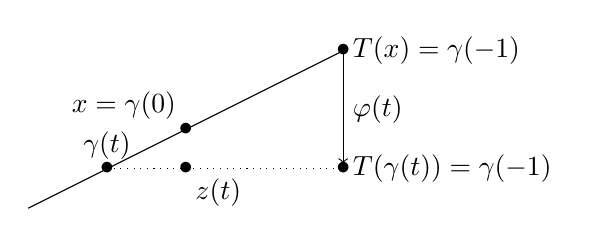
\begin{tikzpicture}
        \draw (-1,-0.5) -- (3,1.5);
        \draw (0,0) node[above] {$\gamma(t)$} node {$\bullet$};
        \draw (1,0.5) node[above left] {$x=\gamma(0)$} node {$\bullet$};
        \draw (3,1.5) node[right] {$T(x)=\gamma(-1)$} node {$\bullet$};
        \draw (3,0) node[right] {$T(\gamma(t))=\gamma(-1)$} node {$\bullet$};
        \draw (1,0) node[below right] {$z(t)$} node {$\bullet$};
        \draw[->] (3,1.5) -- (3,0.07);
        \draw[dotted] (0,0) -- (3,0);
        \draw (3,0.75) node[right] {$\varphi(t)$};
    \end{tikzpicture}
    \caption{Visualization of the defined functions in the proof of Lemma~\ref{Lem:RayConst}.}
    \label{Fig:VisConstRay}
\end{figure}

\begin{proof}[Part 2]
    Now, we extend this argument to the ray from $T(x)$ in direction $x$ that is contained in $\M_\delta$. We again define $\gamma$ and $\varphi$ via:
    $$\gamma(t)\coloneqq x-t(T(x)-x)=(1+t)x-tT(x)$$
    and 
    $$\varphi(t)\coloneqq T(\gamma(t))-T(x).$$
    
    Consider $y$ on this line such that $x$ lies between $y$ and $T(x)$. Then, there is $t^*>0$ such that $y=\gamma(t^*)$. We define a convex combination between $\gamma(t)$ and $T(\gamma(t))$, see Figure~\ref{Fig:VisConstRay} via
    \begin{align*}
        z(t)&=x+\frac{t}{1+t}\varphi(t)=x+\frac{t}{1+t}T(\gamma(t))-\frac{t}{1+t}T(x)\\
        &=\frac{1}{1+t}\gamma(t)+\frac{t}{1+t}T(\gamma(t)).
    \end{align*}
    By the first part, we know $T(z(t))=T(\gamma(t))=\varphi(t)+T(x)$.
    This allows to compute
    \begin{align*}
        \varphi'(t)&=DT(\gamma(t))\gamma'(t)\\
        &=DT(z(t))z'(t)=DT(z(t))\left(\frac{1}{(1+t)^2}\varphi(t)+\frac{t}{1+t}\varphi'(t)\right)
    \end{align*}
    where we used $\left(1-\frac{1}{1+t}\right)'=\frac{1}{(1+t)^2}$.
    Now let $\tau>0$ be such that $\tau\sup\limits_{t\in [0,\tau]}DT(z(t))<\frac{1}{2}$.
    Then, $|\varphi(t)|'\leq \frac{1}{\tau}|\varphi|$ by Grönwall and since $\varphi(0)=0$, we conclude $\varphi\equiv 0$ on $[0,\tau)$ which implies $T(\gamma(t))=T(x)$ on $[0,\tau)$ and by continuity also $T(\gamma(\tau))=T(x)$.

    Now we conclude that $I\coloneqq \{t\in [0,t^*]:\ \varphi(s)=0 \ \text{ for all } s\leq t\}$ is relatively open and closed and contains $0$ which implies $I=[0,t^*]$.
\end{proof}

\begin{corollary}
    Lemma~\ref{Lem:RayConst} implies that $T(T(x)) = T(x)$, so $T$ is an idempotence.
    \label{Cor:T2T}
\end{corollary}

\begin{proof}
    Choosing $s=1$ in Lemma~\ref{Lem:RayConst} gives $T(T(x)) = T(x)$ as desired. 
\end{proof}

\begin{lemma}[Local affine level sets]
    Let $T(y)=T(z)=x$ and let $\Pi$ be the affine plane through $x,y,z$. Then $T(w)=x$ for every
    $w\in\Pi$ for which the segment $[x,w]$ is contained in $\M_\delta$. In particular $T^{-1}(x)$
    contains a relative neighborhood of $x$ in $\Pi$, so the level set through $x$ is locally an
    affine subspace. %Consequently $V(x)=\{ s(y-x) \::\:  y \in \M_\delta, \; \,T(y) = x, \; s >0\}$ is a vector space.
    \label{Lem:AffineLevel}
\end{lemma}

We note specifically that $y=z$ is allowed and $w$ does not have to be a convex combination of
$y$, $z$ and $x$. The hypothesis $[x,w]\subset \M_\delta$ cannot be relaxed to ``$w$ lies in the
connected component of $\Pi\cap \M_\delta$ containing $x$'': such a component need not be
star-shaped about $x$ --- for a circle $\M\subset\mathbb{R}^3$ and $\Pi$ the plane of the circle,
$\Pi\cap \M_\delta$ is an annulus --- and the argument below produces a second direction only at
fixed points of $T$, so it cannot be iterated away from $x$.

\begin{figure}[!ht]
    \centering
    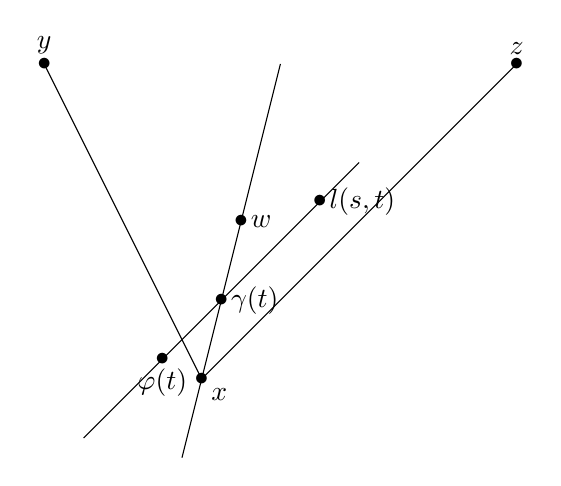
\begin{tikzpicture}
        \draw (0,0) -- (-2,4);
        \draw (-2,4) node[above] {$y$} node {$\bullet$};
        \draw (0,0) -- (4,4);
        \draw (4,4) node[above] {$z$} node {$\bullet$};
        \draw (-0.25,-1) -- (1,4);
        \draw (0,0) node[below right] {$x$} node {$\bullet$};
        \draw (0.5,2) node[right] {$w$} node {$\bullet$};
        \draw (0.25,1) node[right] {$\gamma(t)$} node {$\bullet$};
        \draw (-1.5,-0.75) -- (2,2.75);
        \draw (-0.5,0.25) node[below] {$\varphi(t)$} node {$\bullet$};
        \draw (1.5,2.25) node[right] {$l(s,t)$} node {$\bullet$};
    \end{tikzpicture}
    \caption{Visualization of the proof of Lemma~\ref{Lem:AffineLevel}.}
    \label{Fig:VisConstLine}
\end{figure}

\begin{proof}
We define $v\coloneqq w-x$ which is a linear combination of $y-x$ and $z-x$. Moreover, by Lemma~\ref{Lem:RayConst}, we have $DT(x)(y-x)=DT(x)(z-x)=0$ and thus
$$DT(x)v=0.$$
Moreover, let $\gamma(t)\coloneqq x+tv$ be the ray from $x$ in direction $w$ and $\varphi(t)\coloneqq T(\gamma(t))$ be their images. Then, $\varphi(0)=x, \varphi'(0)=0$ which implies $|\varphi(t)-x|\leq ct^2$.

Now, let $l(s,t)\coloneqq \varphi(t)+s\frac{\gamma(t)-\varphi(t)}{|\gamma(t)-\varphi(t)|}$ be the connection from $\gamma(t)$ to $\varphi(t)$ for $s\in [0,s^*]$ s.t.\ $l(s,t)$ is in $\M_\delta$ for all $s\leq s^*$. Since $x,\varphi(t)\in \M_{\frac{\delta}{2}}$, there is a uniform (in $t$) lower bound on $s^*$. By Lemma~\ref{Lem:RayConst} we have $T(l(s,t))=\varphi(t)$ and since $|\varphi(t)-x|^2\leq ct^2$, we have $l(s,t)\to l(s,0)\coloneqq x+s\frac{v}{|v|}$ uniformly in $s$ on $[0,s*]$. By continuity, we follow $\varphi(t)=T(l(s,t))\to T\left(x+s\frac{v}{|v|}\right)$ as $t\to 0$. But since $\varphi(t)\to x$, we conclude
$$T\!\left(x+s\tfrac{v}{|v|}\right)=x \qquad \text{for } 0\le s\le s^* .$$
As $v$ ranges over the directions of $\Pi$ and $s^*$ is bounded below uniformly, this already shows
that $T\equiv x$ on a relative neighborhood of $x$ in $\Pi$, which is the local affineness asserted.

To reach a general $w$, pick $0<s\le s^*$ and set $p\coloneqq x+s\frac{v}{|v|}$ with $v=w-x$. Then
$T(p)=x$, so by Lemma~\ref{Lem:RayConst} the map $T$ is constant, with value $x$, on the connected
component of $\{x+\sigma v:\sigma\in\mathbb{R}\}\cap \M_\delta$ containing the segment $[x,p]$. If
$[x,w]\subset \M_\delta$ then $w$ belongs to that component, whence $T(w)=x$.
\end{proof}

\begin{corollary}[Lines const]
    Lemma~\ref{Lem:AffineLevel} implies that the connected line through $x$ and $T(x)$ is mapped to $T(x)$.
    \label{Cor:LinesConst}
\end{corollary}

\begin{lemma}[Non-empty level sets]
For all $x\in \widehat{\M}$, there exists some $y\in \overline{\M}_\delta \setminus \widehat{\M}$ such that $T(y)=x$.
\label{Lem:LevelSetNonEmpty}
\end{lemma}

\begin{proof}
    Since we know that $T(T(x))=T(x)$ for all $x$, we conclude that 
    $\widehat{\M} = \{x\in \overline{\M}_\delta:\; T(x)=x\}$.
    % \begin{equation}\label{eqn:OmegaA}
    %     \Omega= T(\overline \M_\delta) = \{x\in \overline{\M}_\delta:\; T(x)=x  \}=:A.
    % \end{equation}
    % According to statement 1, for any $y \in \Omega$ we have $T(y)=y$ and hence $\Omega \subset A$. On the other hand, it is straightforward to show that $A\subset \Omega$, since for any $x\in A$ we have $x =T(x)\subset T(\overline \M_\delta)$. 

    % Note that for any $x\in \Omega^\circ$, there does not exist any $y\in \overline{\M}_\delta$ such that $y\neq x$ and $T(y)=x$. It is clear for the case $y\in \Omega$ since we have $T(y)=y\neq x$. By contrast, if $y \in \overline{\M}_\delta \setminus \Omega$, we proceed by contradiction. Assume that $T(y)=x$, it follows from property (ii) that there exists some $s\in \R\setminus\{0\}$ such that $x + s(y-x) \in \Omega$ satisfies
    % \[ x + s(y-x) = T(x + s(y-x)) = T(x) =x,  \]
    % which implies $y=x$ and therefore leads to a contradiction. Hence, $T(x)=x$ for $x\in \Omega$ and $T(\overline{\M}_\delta \setminus \Omega) \subset \partial \Omega$.

    Next, we proceed to show that for all $x \in \partial \widehat{\M}$, there exists some $y\in \overline{\M}_\delta \setminus \widehat{\M}$ such that $T(y)=x$. Since $x\in \partial \widehat{\M}$ there exists a sequence $z_n \to x$ as $n \to \infty$ and $z_n \in \M_\delta \setminus \widehat{\M}$. Let $x_n =T(z_n)$. By continuity $x_n \to x $ as $n \to \infty$.  Let $y_n = x_n + \veps \frac{z_n - x_n}{|z_n - x_n|}$, where $\veps>0$ is small enough for all of $y_n$ to belong to $\M_\delta$. By Corollary~\ref{Cor:LinesConst}, we have $T(y_n) = x_n$. By compactness of $\overline \M_\delta$
   $y_n$ converges along a subsequence to some $y \in \M_\delta$. Note that $y \neq x$ since $|y-x| \geq \veps$. On the other hand $T(y) = \lim_{n \to \infty} T(y_n) = \lim_{n \to \infty} x_n = x$ as desired. 
    
    
    
    % Since $x\in \partial \Omega$ and $\partial\M_\delta \cap \partial \Omega =\emptyset$, there exist some $z \in \M_\delta \setminus \Omega$ such that the line segment $\overline{xz}$ satisfies $\overline{xz}\cap \Omega=\{x\}$, and some $r>0$ such that the $r$-neighborhood of $\overline{xz}$ is inside the tubular neighborhood $\M_\delta$. Without loss of generality, we also assume that $T(z) \neq x $. 
    % Denote \[\ell(s):=(1-s) x + s z\] as a map onto the line segment $\overline{xz}$. We consider a sequence of points $\{y_n\}_{n=1}^\infty\subset \M_\delta$ defined by
    % \[ y_n: = \ell(n^{-1}) + \frac{ \ell(n^{-1})- T\left(\ell(n^{-1}) \right)}{|\ell(n^{-1})- T\left(\ell(n^{-1}) \right)|}r. \]
    % Then $y_n$ is a point lying in the line passing through $\ell(n^{-1})$ and $T(\ell(n^{-1}))$. It follows from property (ii) that $T(y_n) = T(\ell(n^{-1}))$ for each $n\in \N$. Also, we have $|y_n- \ell(n^{-1})|=r>0$ by definition. Since $\M$ is compact, it is clear that $\{y_n\}_{n=1}^\infty$ is precompact. Therefore, by passing to a subsequence without relabeling, there exists some $y\in \overline{\M}_\delta$ such that $y_{n} \ria y$ as $n$ goes to infinity. Since $T$ is smooth and $\ell(n^{-1}) \ria x$ as $n\ria \infty$, we can compute
    % \[ T(y)=\lim_{n\to \infty} T(y_n) = \lim_{n\to \infty} T(\ell(n^{-1})) = T(x)=x \quad \text{with} \quad |y-x|=\lim_{n\ria \infty}|y_n - \ell(n^{-1})| =r>0.  \]
    % As a sequence, we deduce that there exists some $y\in \overline{\M}_\delta \setminus \Omega$ satisfying $T(y)=x\neq y$.

    To establish the claim, it suffices to show that there is no interior point in $\widehat{\M}$. In this case, we have $\widehat{\M} =\partial \widehat{\M}$. Assume, for the sake of contradiction, that $x_0 \in \widehat{\M}^\circ$, then there exists an inscribed ball $B(x_0, r_0)\subset \widehat{\M}$ in $\mathbb{R}^D$ that touches the boundary at a point $x\in \partial \widehat{\M}$. More precisely, one can choose $r_0=d(x_0, \partial \widehat{\M})$. By the previous observation, there exists some $z \in \overline{\M}_\delta \setminus \widehat{\M}$ such that $T(z)=x$. 

    Denote $\ell_{xz}$ as the line passing through $x$ and $z$. We separate the analysis depending on the intersection between the line $\ell_{xz}$  and the inscribed ball $B(x_0, r_0)$. Suppose $\ell_{xz}\cap B(x_0, r_0) = \{x\}$, that is, $\ell_{xz}$ is tangent to $B(x_0, r_0)$, similarly we consider a point $\ell(s)$ in the line segment $\overline{xz}$. Define $P_B: \ell_{xz} \mapsto \partial B(x_0, r_0)$ by
    \[ P_B(y) : =  \mathop{\arg\min}\limits_{\omega\in W}|y-\omega| \q \text{where} \q W:=\{ \partial B(x_0, r_0) \cap (y + t(x -x_0)):\; t\in \mathbb{R} \}. \]
    Then $P_B$ is a parallel projection from the line $\ell_{xz}$ onto the inscribed ball along the radial direction $\overline{x x_0}$. Applying Corollary~\ref{Cor:LinesConst} gives, for $0 < s \ll 1$,
    \[ T(\ell(s))=x \q \text{and} \q T(P_B(\ell(s))) = P_B(\ell(s)). \]
    Since the sphere lies quadratically below the tangent plane, one can find that 
    \[ \frac{|T(P_B(\ell(s))) - T(\ell(s))|}{| P_B(\ell(s)) - \ell(s)|} = \frac{|P_B(\ell(s)) - x|}{|P_B(\ell(s)) - \ell(s)|} \to \infty \q \text{as} \q s \to 0, \]
    which leads to a contradiction as the left hand side term is bounded by the Lipschitz constant of $T$. More precisely, a direct computation via orthogonality gives
    \[ |P_B(\ell(s)) - x|^2 =2 r_0 |P_B(\ell(s)) - \ell(s)|\]
    and 
    \[ |P_B(\ell(s)) - x|^2 - |P_B(\ell(s)) - \ell(s)|^2 =|x-\ell(s)|^2 = s^2 |x-z|^2.  \]
    Combining these formulae together yields
    \[ \frac{|P_B(\ell(s)) - x|}{|P_B(\ell(s)) - \ell(s)|} = \sqrt{\frac{2 r_0}{r_0 - \sqrt{r_0^2 -s^2|x-z|^2}}} \to \infty \q \text{as} \q s \to 0.\]

    For the other case $\ell_{xz}\cap B(x_0, r_0) \neq \{x\}$, it implies that there exist some point $z_0 \in \ell_{xz}\cap B(x_0, r_0)$ with $z_0\neq x$. This does not hold since we have $T(z_0)=z_0$ and $T(z_0)=x$ by Corollary~\ref{Cor:LinesConst} at the same time. This completes the proof.
\end{proof}

\begin{comment}
\begin{lemma}[stronger version of (image of preimage) needed below]
    Every $x\in \Omega$ has an open neighborhood $U$ in $\Omega$ such that $T^{-1}(U)$ is an open set in $\overline \M_\delta$ and is homeomorphic to $U \times \overline B_k$.
    \label{Lem:PreimageImage}
\end{lemma}
\end{comment}

\begin{proposition}[Constant rank of $T$]
    Let $U$ be an open connected set and $T\in C^1(U)$ a projection in the sense that $T=T^2$. Then $DT$ has constant rank on the image of $T$.
    \label{Prop:ConstRk}
\end{proposition}

\begin{proof}
    Since $T$ is idempotent, we can compute the derivative of the identity on the image of $T$. Let $y\in \widehat{\M}$. Then $T(y)=y$ and thus
    \begin{align*}
        DT(y)=DT(T(y))\cdot DT(y)=DT^2(y).
    \end{align*}
    Hence, $DT$ is an idempotent matrix on the image of $T$ which especially implies $\text{rank}(DT)=\text{tr}(DT)$. The trace is a continuous map and the rank a discrete map. Therefore, the rank has to be constant on $\widehat{\M}$ as it is connected.
\end{proof}

\begin{lemma}[Globally constant rank]
    The rank of $DT$ is constant on $\M_\delta$.
    \label{Lem:RankTAll}
\end{lemma}

\begin{proof}
    Let $k$ denote the rank of $DT$ on $\widehat \M$, which is constant by
    Proposition~\ref{Prop:ConstRk}. Fix $y\in \M_\delta$ and set
    \[
        \Phi_t(y)\coloneqq (1-t)y+tT(y), \qquad t\in[0,1].
    \]
    By Proposition~\ref{Prop:StarShaped} we have $\Phi_t(y)\in \M_\delta$, and by
    Lemma~\ref{Lem:RayConst},
    \[
        T(\Phi_t(y))=T(y) \qquad \text{for every } y\in \M_\delta .
    \]
    For fixed $t$ this is an identity between maps on the open set $\M_\delta$, so it may be
    differentiated in $y$. Since $D\Phi_t(y)=(1-t)I+t\,DT(y)$, we obtain
    \begin{equation}\label{eqn:rankidentity}
        DT\bigl(\Phi_t(y)\bigr)\,\bigl[(1-t)I+t\,DT(y)\bigr] \;=\; DT(y),
        \qquad t\in[0,1].
    \end{equation}

    \emph{Upper bound.} Taking $t=1$ in \eqref{eqn:rankidentity} gives $DT(T(y))\,DT(y)=DT(y)$,
    and therefore
    \[
        \mathrm{rank}\,DT(y)\;\le\;\mathrm{rank}\,DT(T(y))\;=\;k,
    \]
    since $T(y)\in\widehat \M$.

    \emph{Lower bound.} The map $t\mapsto \det\bigl((1-t)I+t\,DT(y)\bigr)$ is a polynomial of
    degree at most $D$ taking the value $1$ at $t=0$; it is thus not identically zero and vanishes
    for at most $D$ values of $t$. For every other $t$ the bracket in \eqref{eqn:rankidentity} is
    invertible, so that
    \[
        \mathrm{rank}\,DT\bigl(\Phi_t(y)\bigr)\;=\;\mathrm{rank}\,DT(y).
    \]
    Choose such $t_j\uparrow 1$. Then $\Phi_{t_j}(y)\to T(y)\in\widehat \M$, and since the rank is
    lower semicontinuous --- the sets $\{\mathrm{rank}\,DT\le m\}$ are closed, being the common
    zero sets of all $(m+1)$-minors of $DT$ --- we conclude
    \[
        \mathrm{rank}\,DT(y)\;=\;\liminf_{j\to\infty}\mathrm{rank}\,DT\bigl(\Phi_{t_j}(y)\bigr)
        \;\ge\;\mathrm{rank}\,DT(T(y))\;=\;k .
    \]

    The two bounds give $\mathrm{rank}\,DT(y)=k$ for every $y\in \M_\delta$.
\end{proof}

\begin{proposition}[Image is a closed $C^2$ manifold]
    $\widehat{\M}$ is a compact $C^2$ embedded submanifold of $\mathbb{R}^D$ without boundary, of
    dimension $k=\mathrm{rank}\,DT$.
    \label{Prop:SmoothManifoldImage}
\end{proposition}

\begin{proof}
    \emph{Compactness.} By Corollary~\ref{Cor:T2T} we have
    $\widehat \M=\{x\in\overline{\M_\delta}:T(x)=x\}$. No fixed point lies on $\partial \M_\delta$:
    if $x\in\partial \M_\delta$ then $d_\M(x)=\delta$, whereas $E_3(T)=0$ forces
    $T(x)\in\overline{\M_{\frac{\delta}{2}}}$, so $T(x)\neq x$. Consequently
    $T(\M_\delta)=T(\overline{\M_\delta})=\widehat \M$, and $\widehat \M$ is compact as the continuous
    image of a compact set. In particular $\widehat \M\subset \M_\delta$.

    \emph{Manifold structure.} By Proposition~\ref{Prop:ConstRk} and Lemma~\ref{Lem:RankTAll} the
    rank of $DT$ equals a constant $k$ on all of $\M_\delta$. Let $y\in\widehat \M$. By the constant
    rank theorem there are charts around $y$ and around $T(y)=y$ in which $T$ takes the form
    \[
        (x_1,\dots,x_D)\;\longmapsto\;(x_1,\dots,x_k,0,\dots,0)
    \]
    on some open neighborhood $U\subset \M_\delta$ of $y$. Hence $T(U)$ is a $k$-dimensional
    embedded submanifold of $\mathbb{R}^D$ which is diffeomorphic to an open subset of
    $\mathbb{R}^k$; in particular it has no boundary.

    It remains to see that $T(U)$ describes $\widehat \M$ near $y$. On the one hand
    $T(U)\subseteq T(\M_\delta)=\widehat \M$. On the other hand, if $z\in \widehat \M\cap U$ then
    $T(z)=z$ and therefore $z\in T(U)$. Consequently
    \[
        \widehat \M\cap U \;=\; T(U)\cap U ,
    \]
    which is an open subset of the boundary-less $k$-manifold $T(U)$, and a relatively open
    neighborhood of $y$ in $\widehat \M$. Since $y\in\widehat \M$ was arbitrary, $\widehat \M$ is a
    $k$-dimensional embedded submanifold without boundary.
\end{proof}

\begin{proposition}[Deformation retract implies dimension]
    Let $N_1,N_2$ be closed connected $C^2$ manifolds, that is, compact, connected and without
    boundary, and let $U\subset\mathbb{R}^D$ be a set containing them such that there exist
    deformation retracts of $U$ onto $N_1$ and onto $N_2$. Then $\dim N_1=\dim N_2$.
    \label{Prop:DeformationRetract}
\end{proposition}

Neither hypothesis can be dropped, and it is the absence of boundary that does the work. The
criterion used below is specific to closed manifolds: a compact connected $m$-manifold with
non-empty boundary has $H_m=0$, being homotopy equivalent to a CW complex of dimension at most
$m-1$, so its top non-vanishing homology no longer detects $m$. For instance $U=\mathbb{R}^D$
deformation retracts onto $\{0\}$ and also onto the closed unit ball $\overline{B^D}$, by
$H(x,t)=x$ for $|x|\le 1$ and $H(x,t)=\left((1-t)+\frac{t}{|x|}\right)x$ for $|x|\ge 1$; both retracts are
compact and connected, of dimensions $0$ and $D$. Dropping compactness fails for the same reason,
as $\mathbb{R}^D$ is itself a deformation retract of $U=\mathbb{R}^D$.

\begin{proof}
    A deformation retract of $U$ onto $N_1$ makes $N_1$ and $U$ homotopy equivalent, and likewise
    for $N_2$, so that $H_j(N_1)\cong H_j(U)\cong H_j(N_2)$ for every $j$.

    For a closed connected manifold $N$ of dimension $m$ one has $H_j(N)=0$ for all $j>m$, together
    with $H_m(N)\cong\mathbb{Z}$ if $N$ is orientable, and $H_m(N)=0$ while $H_{m-1}(N)$ contains
    $\mathbb{Z}_2$ as its torsion subgroup if $N$ is not orientable. In either case the dimension
    is determined by the homology: it is the largest $j$ with $H_j(N)\neq 0$ in the orientable
    case, and one more than that in the non-orientable case, the two being distinguished by whether
    the top non-vanishing group is $\mathbb{Z}$ or has $\mathbb{Z}_2$-torsion. Since $N_1$ and
    $N_2$ have isomorphic homology they fall into the same case and have the same dimension.
\end{proof}

\begin{proposition}[Image of $T$ is $\M$]
    \label{Prop:ImTM}
    The image $\widehat{\M}$ of $\overline{\M_\delta}$ under $T$ is $\M$.
\end{proposition}

\begin{proof}[Proof of Proposition~\ref{Prop:ImTM}]
    By Lemma~\ref{Lem:EasyProp} we have $T=\mathrm{Id}$ on $\M$, hence $\M\subseteq\widehat \M$.

    \emph{Both sets are deformation retracts of $\M_\delta$.} By Proposition~\ref{Prop:StarShaped}
    the segment $[x,T(x)]$ lies in $\M_\delta$ for every $x\in \M_\delta$, so
    $H(x,t)\coloneqq(1-t)x+tT(x)$ maps $\M_\delta\times[0,1]$ into $\M_\delta$; it satisfies
    $H(\cdot,0)=\mathrm{Id}$, $H(\cdot,1)=T$ with image $\widehat \M$, and $H(y,t)=y$ for
    $y\in\widehat \M$ because $T(y)=y$. Thus $H$ is a deformation retract of $\M_\delta$ onto
    $\widehat \M$. Likewise 
    $$\widetilde H(x,t)\coloneqq(1-t)x+t\pi_\M(x)$$
    is a deformation retract of
    $\M_\delta$ onto $\M$: every point of the segment $[x,\pi_\M(x)]$ is at distance at most
    $d_\M(x)<\delta$ from $\M$, and $\pi_\M$ fixes $\M$ pointwise.

    \emph{Equal dimensions.} The manifold $\M$ is closed and connected by assumption, and
    $\widehat \M$ is closed and connected by Proposition~\ref{Prop:SmoothManifoldImage} together
    with Lemma~\ref{Lem:EasyProp}. Proposition~\ref{Prop:DeformationRetract} therefore applies and
    gives $\dim\widehat \M=\dim \M=d$.

    \emph{Conclusion.} Now $\M\subseteq\widehat \M$ are both $d$-dimensional embedded submanifolds
    without boundary, so the inclusion $\M\hookrightarrow\widehat \M$ is a continuous injection
    between manifolds of equal dimension and is therefore open, by invariance of domain. Hence $\M$
    is open in $\widehat \M$. It is also closed in $\widehat \M$, being compact, and it is non-empty.
    Since $\widehat \M$ is connected, $\M=\widehat \M$.
\end{proof}

\begin{proof}[Proof of Theorem~\ref{Thm:TPiM}]
For any $x\in \partial \M_\delta$, it is clear that $d(x, \M)=\delta$. By Proposition~\ref{Prop:ImTM}, we have $T(x) \in \M$, then it follows from the last item of Lemma~\ref{Lem:EasyProp} that 
\[ \delta \ge |T(x) - x| \ge d(x, \M) =\delta \ra |T(x) - x| = d(x, \M) =\delta, \]
which implies $T(x) = \pi_\M (x)$ for any $x\in \partial \M_\delta$.

On the other hand, let $x \in \M_\delta \setminus \M$, again we have $y = T(x) \in \M$. Denote $z:= x + s(y-x)$ for some $s \in \mathbb{R}$. Since $\M$ is compact and $|z-y|=|s-1||x-y|$ with $|x-y|\neq 0$, it follows from Corollary~\ref{Cor:LinesConst} that there exists some $s<0$ such that $z\in \partial \M_\delta$ satisfying $\pi_\M(z) = T(z)=y$. According to the properties of orthogonal projection, we can compute
\[ |z-x| + |x - y| = |z- y| = |z- \pi_\M(z)| \le |z- \pi_\M(x)| \le |z-x| + |x - \pi_\M(x)|,   \]
which implies $|x- T(x)| = |x-y| \le |x - \pi_\M(x)|$ and hence $T(x) = \pi_\M(x)$ by the uniqueness of the nearest point on the manifold. Thus, we conclude with the first item of Lemma~\ref{Lem:EasyProp} that $T(x) = \pi_\M(x)$ for all $x\in \overline{\M}_\delta$.
\end{proof}

\section{Finite \texorpdfstring{$n$}{n} Analysis} \label{sec:finite_n}
\label{Sec:FiniteNAnalysis}

\medskip
\noindent Throughout this section $h$ denotes the \emph{covering radius} of the sample in $\M$,
\[
    h \;\coloneqq\; \max_{z\in \M} d(z, \M_n),
\]
and we assume \eqref{eqn:slackhyp}, i.e.\ $h\le\underline\delta\le\frac{\delta}{8}$, together with
$\mathrm{reach}(\M)\ge 10\delta$. Two elementary inclusions are used
repeatedly. Since $\M_n\subset \M$ one has $d_\M\le d_{\M_n}$ and therefore
\begin{equation}\label{eqn:tubeincl1}
    \M_{n,s}\subseteq \M_s \qquad\text{for every } s>0 .
\end{equation}
Conversely, let $d_\M(u)=t$, put $p=\pi_\M(u)$ and let $X_i$ be a sample with $|p-X_i|\le h$. The
vector $p-X_i$ is a chord of $\M$, hence tangential up to $\frac{h^2}{2\,\mathrm{reach}(\M)}$, so that
\[
    |u-X_i|^2\;=\;|u-p|^2+|p-X_i|^2+2\langle u-p,\,p-X_i\rangle
    \;\le\; t^2+h^2\Bigl(1+\frac{t}{\mathrm{reach}(\M)}\Bigr).
\]
Consequently $u\in \M_{n,\delta}$ whenever $t\le\delta'$, where
\begin{equation}\label{eqn:tubeincl2}
    \delta'\;\coloneqq\;\sqrt{\delta^2-h^2\Bigl(1+\frac{\delta}{\mathrm{reach}(\M)}\Bigr)} ,
    \qquad\text{so that}\qquad \M_{\delta'}\subseteq \M_{n,\delta} .
\end{equation}
The shrinking is only \emph{quadratic} in the covering radius,
\begin{equation}\label{eqn:tubegap}
    \delta-\delta'\;\approx\;\frac{1}{2\delta}\Bigl(1+\frac{\delta}{\mathrm{reach}(\M)}\Bigr)h^2 ,
\end{equation}
because displacing a sample tangentially by $h$ costs only $\mathcal{O}(\frac{h^2}{\delta})$ in the radial direction.
This is the source of the exponent $n^{-\frac{2}{d}}$ in what follows, and it is considerably sharper than
the naive inclusion $\M_{\delta-h}\subseteq \M_{n,\delta}$.

\medskip
\noindent We write $\eta\coloneqq\delta-\delta'$ for this gap. Under the standing assumptions it is
a small fraction of $\delta$: with $\kappa\coloneqq\frac{\delta}{\mathrm{reach}(\M)}\le\frac{1}{10}$ one has
$\delta'\ge\delta\sqrt{1-\frac{1+\kappa}{64}}\ge0.99\,\delta$, so
\begin{equation}\label{eqn:etasmall}
    \eta\;=\;\frac{h^2(1+\kappa)}{\delta+\delta'}
    \;\le\;\frac{\frac{\delta^2}{64}\,(1.1)}{1.99\,\delta}\;\le\;\frac{\delta}{100} .
\end{equation}

\medskip
\noindent The main result of this section is Theorem~\ref{Thm:FiniteN} below: for a minimizer $T_n$
of $E_n$, the energy vanishes, the image $\widehat{\M}_n$ is a compact $C^2$
manifold without boundary containing the sample, it lies within $O\left(\frac{h^2}{\delta}\right)$ of $\M$, and
$\pi_\M$ restricted to it is a homotopy equivalence onto $\M$, so that
$d_\calH(\widehat{\M}_n,\M)=O\left(\frac{h^2}{\delta}\right)$. No bound on the reach of $\widehat{\M}_n$ is asserted: an
unconditional one is false by Remarks~\ref{Rem:noReach} and~\ref{Rem:noTangentBound}, and the reach
is recovered only under a bound on $D^2T_n$, in Proposition~\ref{Prop:ReachC2}. Its proof follows
the population argument of
Section~\ref{Sec:Projection} step by step, with one substitution and one genuinely new ingredient.

\emph{Zero energy} is obtained exactly as in Lemma~\ref{Lem:EasyProp}, testing with $\pi_\M$. Indeed
$E_{1,n}(\pi_\M)=0$ because $X_i\in \M$; $E_{2,n}(\pi_\M)=0$ because
$D\pi_\M(x)(\pi_\M(x)-x)=0$, which is legitimate on $\M_{n,\delta}\subseteq \M_\delta$
by~\eqref{eqn:tubeincl1}; and $E_{4,n}(\pi_\M)=0$ because $|x-\pi_\M(x)|=d_\M(x)<\delta$. The 
only term needing the covering hypothesis is $E_{3,n}$: for $x\in \M_{n,\delta}$ the point
$\pi_\M(x)$ lies in $\M$, hence within $h\le\underline\delta$ of the sample by \eqref{eqn:slackhyp},
so $d_{\M_n}(\pi_\M(x))\le \underline\delta$ and $E_{3,n}(\pi_\M)=0$.

\emph{The consequences of zero energy} are those of Lemma~\ref{Lem:EasyProp} with $\M$ replaced by
$\M_n$ in the first item only:
\begin{itemize}
    \item $T_n(X_i)=X_i$ for every $i$, so $\M_n\subseteq\widehat{\M}_n$;
    \item $DT_n(x)(T_n(x)-x)=0$ on $\M_{n,\delta}$;
    \item $\mathrm{range}(T_n)\subseteq\overline{\M_{n,\underline\delta}}$, so that $$d_\M(T_n(x))\le d_{\M_n}(T_n(x))\le\underline\delta\le\frac{\delta}{8};$$
    \item and $|x-T_n(x)|\le\delta$.
\end{itemize}

\emph{The new ingredient} is the analogue of Proposition~\ref{Prop:StarShaped}. Its population
proof cannot be transplanted: it is a statement about the level sets of $d_\M$, and the corresponding
statement for $d_{\M_n}$ would require $\mathrm{reach}(\M_n)\gtrsim\delta$, whereas
\[
    \mathrm{reach}(\M_n)=\tfrac12\min_{i\neq j}|X_i-X_j| \;\asymp\; n^{-\frac{2}{d}} \;\ll\; \delta .
\]
 We therefore prove the segment property on the shrunken tube instead.

\begin{lemma}[Star-shapedness on the shrunken tube]
    \label{Lem:StarShapedDiscrete}
    Assume \eqref{eqn:slackhyp} and $\mathrm{reach}(\M)\ge 10\delta$. Then for every
    $x\in \M_{\delta'}$ the segment $[x,T_n(x)]$ is contained in $\M_{\delta'}$.

    In particular $H_t\coloneqq(1-t)\,\mathrm{Id}+t\,T_n$ maps $\M_{\delta'}$ into itself for every
    $t\in[0,1]$.
\end{lemma}

\begin{remark}
    The hypothesis is $x\in \M_{\delta'}$ and \emph{not} $x\in\M_{n,\delta'}$, although the latter
    is the smaller set by \eqref{eqn:tubeincl1}. This matters: the conclusion places the segment in
    $\M_{\delta'}$, so only the formulation above produces a homotopy of a set into itself, which is
    what the deformation-retract argument for the dimension of $\widehat{\M}_n$ requires. It has
    the further advantage that $\M_{\delta'}$ deformation retracts onto $\M$ through $\pi_\M$, since
    $\delta'<\mathrm{reach}(\M)$, so that the homotopy type of the domain is available at once; on
    the union of balls $\M_{n,\delta'}$ one would instead have to invoke the
    Niyogi--Smale--Weinberger reconstruction theorem.
\end{remark}

\begin{proof}
    By \eqref{eqn:tubeincl2} we have $\M_{\delta'}\subseteq\M_{n,\delta}$, so the consequences of
    zero energy are available at $x$. The endpoints lie in $\M_{\delta'}$: $d_\M(x)\le\delta'$ by
    hypothesis, and $d_\M(T_n(x))\le\underline\delta\le\frac{\delta}{8}\le\delta'$.

    Suppose the segment left $\M_{\delta'}$. Write $r=|x-T_n(x)|\le\delta$,
    $\tau=\frac{x-T_n(x)}{r}$ and $d(t)=d_\M(T_n(x)+t\tau)$ as in the proof of
    Proposition~\ref{Prop:StarShaped}, so that $d(0)\le\frac{\delta}{8}$, $d(r)\le\delta'$ and $d$ exceeds
    $\delta'$ somewhere in between. Exactly as there, there are $\widetilde t<t_2$ with
    \[
        d'(\widetilde t)\;\ge\;\frac{\delta'-\frac{\delta}{8}}{r}\;\ge\;\frac{\delta'-\frac{\delta}{8}}{\delta}
        \;\ge\;\frac{0.99-0.125}{1}\;\ge\;\frac14 ,
        \qquad d'(t_2)<0,
    \]
    using $\delta'\ge0.99\,\delta$ and $r\le\delta$; hence some $t'$ has
    $d''(t')<-\tfrac{1}{4\delta}$. The computation of Proposition~\ref{Prop:StarShaped} then
    produces a principal curvature of $\partial \M_{d_\M(x')}$ below $-\tfrac{1}{4\delta}$, so that
    $\mathrm{reach}(\M_{d_\M(x')})<4\delta$. Since $d_\M(x')\le\delta$ and, by
    \eqref{eqn:reachtube}, $\mathrm{reach}(\M)=\mathrm{reach}(\M_{d_\M(x')})+d_\M(x')$, this gives
    $\mathrm{reach}(\M)<4\delta+\delta=5\delta$, a contradiction.

    Finally $\M_{\delta'}\subseteq \M_{n,\delta}$ by \eqref{eqn:tubeincl2}.
\end{proof}

\begin{proposition}[fibers are almost normal, and their base points almost lie on $\M$]
    \label{Prop:fiberNormal}
    Assume $\mathrm{reach}(\M)\ge 10\delta$ and \eqref{eqn:slackhyp}. Let $T_n$ be a minimizer of
    $E_n$, let $x\in\M_{n,\delta'}$ and set $w\coloneqq T_n(x)$,
    $a\coloneqq d_\M(w)$, $p\coloneqq\pi_\M(w)$ and $\eta\coloneqq\delta-\delta'$. The fiber through
    $x$ is locally affine by Lemma~\ref{Lem:AffineLevel}; let $F\coloneqq\ker DT_n(x)$ be the linear
    subspace of which it is a translate, and set
    $\beta\coloneqq\max\{\measuredangle(v,N_p\M):v\in F,\ |v|=1\}$. Then
    \[
        a\;\le\;9\,\eta\;\lesssim\;\frac{h^2}{\delta},
        \qquad
        \sin\beta\;\le\;5\sqrt{\frac{\eta}{\delta}}\;\lesssim\;\frac{h}{\delta}.
    \]
    Consequently, $\displaystyle\sup_{y\in\widehat{\M}_n}d(y,\M)\lesssim \frac{h^2}{\delta}\asymp \frac{n^{-\frac{2}{d}}}{\delta}$.
\end{proposition}
\todo[inline]{if $h$ is the fill distance, there has to be additional logarithmic factors and probability}

\begin{remark}[what this proposition does \emph{not} give]
    \label{Rem:noTangentBound}
    An earlier version concluded in addition that $T_y\widehat{\M}_n$ lies within $O\left(\frac{h}{\delta}\right)$
    of $T_p\M$, on the ground that $T_y\widehat{\M}_n=\mathrm{im}\,DT_n(y)$ is complementary to
    $\ker DT_n(y)=F$ and that $F$ is within $\beta$ of $N_p\M$. That inference is false:
    complementarity does not determine a subspace. Take $\M$ closed with
    $\mathrm{reach}(\M)\ge10\delta$, let $g:\M\to N\M$ be $C^2$ with $g(X_i)=0$ and
    $|g(p)|\lesssim \frac{d(p,\M_n)^2}{2\delta}$, and set
    \[
        T_n(x)\;\coloneqq\;\pi_\M(x)+g\bigl(\pi_\M(x)\bigr),\qquad x\in\M_{n,\delta}.
    \]
    Then $T_n$ is constant on the normal fibers of $\M$, so $E_{2,n}=0$ and $F=N_p\M$ exactly,
    i.e.\ $\beta=0$; $E_{1,n}=0$ since $g$ vanishes on the sample; $E_{3,n}=0$ since
    $d_{\M_n}(p+g(p))\le h+|g|\le\underline\delta$; and $E_{4,n}=0$ by the bound on $|g|$,
    which is exactly the quadratic gap $\eta$. So $T_n$ is a zero-energy minimizer. Its image is
    the graph $\{p+g(p)\}$, whose tangent spaces are tilted from $T_p\M$ by $\|Dg\|$ --- and $g$ is
    free to oscillate, since midway between samples the constraint permits $|g|\asymp \frac{h^2}{\delta}$
    on a region of diameter $\asymp h$. Choosing wavelength $\lambda\ll h$ there makes $\|Dg\|$,
    and with it the tilt, arbitrarily large.
\end{remark}

\begin{proof}
    Throughout put $\sigma\coloneqq\sin\beta$, $A\coloneqq \frac{a}{\delta}$ and $\kappa\coloneqq\frac{\delta}{\tau}$
    with $\tau=\mathrm{reach}(\M)$, so $\kappa\le\frac{1}{10}$. Write $n_0\coloneqq w-p$, $|n_0|=a$.

    \emph{The exit constraint.} Let $v$ be a unit vector in $F$, oriented so that
    $\langle n_0,v\rangle\ge0$. In Step~1 below $v$ is chosen to \emph{realize} the maximal tilt,
    $\measuredangle(v,N_p\M)=\beta$, so that $|v_N|=\cos\beta$ exactly; in Step~2 it is chosen aligned with
    $n_0$. In both cases $|v_T|\le\sigma$, which is all that the curvature correction needs. By Corollary~\ref{Cor:LinesConst} the whole connected segment of
    $w+\R v$ inside $\M_{n,\delta}$ maps to $w$, and $E_{4,n}(T_n)=0$ bounds it in
    $\overline{B(w,\delta)}$; by \eqref{eqn:tubeincl2} it must therefore leave $\M_{\delta'}$ at some
    $-s$ with $0<s\le\delta$. Since $\M$ deviates from $p+T_p\M$ by at most
    $\frac{|\cdot|^2}{2\tau}$, writing $v=v_N+v_T$ for the decomposition along $N_p\M\oplus T_p\M$,
    \begin{equation}\label{eqn:exitconstraint}
        \delta'\;\le\;d_\M(w-sv)\;\le\;\bigl|n_0-s\,v_N\bigr|+\frac{s^2|v_T|^2}{2\tau}
        \;\le\;\bigl|n_0-s\,v_N\bigr|+\frac{\delta^2\sigma^2}{2\tau}.
    \end{equation}

    \emph{Step 1: a crude bound.} Take $v$ realizing the maximal tilt, so $|v_N|=\cos\beta$.
    Discarding $-2s\langle n_0,v_N\rangle\le0$ and using $s\le\delta$ gives
    $|n_0-sv_N|\le\sqrt{a^2+\delta^2\cos^2\beta}\le a+\delta\cos\beta$, so
    \eqref{eqn:exitconstraint} yields
    $\delta-\eta\le a+\delta(1-\frac{\sigma^2}{2})+\frac{\delta^2\sigma^2}{2\tau}$, that is
    \begin{equation}\label{eqn:tiltbound}
        \sigma^2\;\le\;\frac{2(a+\eta)}{\delta\,(1-\kappa)} .
    \end{equation}
    Now $E_{3,n}(T_n)=0$ gives $a\le d_{\M_n}(w)\le\underline\delta\le\frac{\delta}{8}$, and
    $\eta\le\frac{\delta}{100}$, so
    \[
        \sigma^2\;\le\;\frac{2\bigl(\tfrac18+\tfrac1{100}\bigr)}{\tfrac9{10}}\;\le\;0.30 ,
        \qquad\text{hence}\qquad \cos\beta\;\ge\;\sqrt{0.70}\;\ge\;\tfrac12 ;
    \]
    we record $\cos\beta\ge\frac{1}{2}$. This is the one place where the size of the slack matters: with
    the population value $\underline\delta=\frac{\delta}{2}$ the right-hand side exceeds $1$ and the
    estimate is vacuous, so the bootstrap could not start. Hypothesis \eqref{eqn:slackhyp} is
    exactly what is needed here.

    \todo[inline]{we use the dimension of $F$ here, so from a presentation standpoint, this proposition or proof should come after that is established and link to the statement}
    \emph{Step 2: the aligned direction.} As $\cos\beta\ge\frac{1}{2}$ and $\dim F=\dim N_p\M$, every unit
    vector of $N_p\M$ makes an angle at most $\beta$ with $F$; in particular there is a unit
    $v\in F$ with $\langle \frac{n_0}{a},v\rangle\ge\cos\beta$. For this $v$,
    \[
        |n_0-sv_N|^2 = a^2-2s\langle n_0,v_N\rangle+s^2|v_N|^2
        \le \delta^2\Bigl(1-2A\cos\beta+A^2\Bigr),
    \]
    and $\sqrt{1+x}\le1+\frac{x}{2}$ gives $|n_0-sv_N|\le\delta-a\cos\beta+\frac{a^2}{2\delta}$. Substituting into
    \eqref{eqn:exitconstraint} and using $A\le\frac{1}{2}$,
    \begin{equation}\label{eqn:distbound}
        a\Bigl(\cos\beta-\tfrac14\Bigr)\;\le\;\eta+\frac{\delta^2\sigma^2}{2\tau}
        \qquad\Longrightarrow\qquad
        a\;\le\;4\eta+\frac{2\delta^2\sigma^2}{\tau},
    \end{equation}
    using $\cos\beta\ge\frac{1}{2}$.

    \emph{Step 3: closing the loop.} Insert \eqref{eqn:tiltbound} into \eqref{eqn:distbound}:
    \[
        a\;\le\;4\eta+\frac{2\delta^2}{\tau}\cdot\frac{2(a+\eta)}{\delta(1-\kappa)}
        \;=\;4\eta+\frac{4\kappa}{1-\kappa}\,(a+\eta)
        \;\le\;4\eta+\tfrac12(a+\eta),
    \]
    since $\kappa\le\frac{1}{10}$ gives $\frac{4\kappa}{1-\kappa}\le\frac{4}{9}<\frac{1}{2}$. Hence $a\le9\eta$, and
    \eqref{eqn:tiltbound} then gives $\sigma^2\le \frac{2\cdot10\eta}{\delta\cdot\tfrac9{10}}\le25\frac{\eta}{\delta}$.

    Finally $\eta=\delta-\delta'\approx \frac{1+\kappa}{2\delta}h^2$ by \eqref{eqn:tubegap}, giving the
    stated orders. Every $y\in\widehat{\M}_n$ is of the form $T_n(x)$, whence the bound on
    $d(y,\M)$.
\end{proof}

\begin{remark}
    Both conclusions come from the single constraint \eqref{eqn:exitconstraint}, applied twice: to
    an arbitrary fiber direction for the tilt, and to the direction aligned with $w-p$ for the
    distance. The bootstrap of Step~3 is necessary because the curvature correction
    $\frac{\delta^2\sigma^2}{2\tau}$ is not small until $\sigma$ is, and it is what forces
    $\mathrm{reach}(\M)\ge10\delta$ rather than $5\delta$.

    What does the work is that $E_{4,n}$ caps the fiber at length $\delta$, that the fiber is
    a full line segment through $w$ rather than a ray, and that it must escape a tube of radius
    $\delta'$ on the far side: it has to spend $a$ reaching $\M$ and a further $\delta'$ getting out,
    while only $\delta$ is available. No regularity of $T_n$ beyond zero energy is used.
\end{remark}

\begin{remark}[no unconditional bound on the reach of $\widehat{\M}_n$]
    \label{Rem:noReach}
    Zero energy gives no lower bound on $\mathrm{reach}(\widehat{\M}_n)$, and the example of
    Remark~\ref{Rem:noTangentBound} already shows it. There $T_n=\pi_\M+g\circ\pi_\M$ is a
    zero-energy minimizer for every admissible $g$, and its image is the graph
    $\{p+g(p):p\in\M\}$. Midway between samples the constraints leave $g$ free on a region of
    diameter $\asymp h$ subject only to $|g|\lesssim \frac{h^2}{\delta}$, so $g$ may be taken with
    amplitude $\varepsilon\asymp \frac{h^2}{\delta}$ and wavelength $\lambda$ as small as one likes. A graph
    of amplitude $\varepsilon$ and wavelength $\lambda$ has curvature $\asymp\frac{\varepsilon}{\lambda^2}$, so
    \[
        \mathrm{reach}\bigl(\widehat{\M}_n\bigr)\;\lesssim\;\frac{\lambda^2}{\varepsilon}
        \;\asymp\;\frac{\lambda^2\,\delta}{h^2}\;\xrightarrow[\ \lambda\to0\ ]{}\;0 ,
    \]
    while $\widehat{\M}_n$ stays within $O\left(\frac{h^2}{\delta}\right)$ of $\M$ throughout.

    The obstruction is one of scale rather than of position. The energy controls how far the image
    lies from $\M$, and \eqref{eqn:tubegap} fixes that distance at $\mathcal{O}(\frac{h^2}{\delta})$; it says nothing
    about the frequency at which the image may oscillate within that band, and reach is a
    second-order quantity. No sharpening of the zero-energy analysis can therefore produce a reach
    bound: control of $D^2T_n$ has to come from outside the variational problem, and what such
    control buys is the content of Proposition~\ref{Prop:ReachC2}.
\end{remark}

\begin{theorem}[Structure of the minimizer at finite $n$]
    \label{Thm:FiniteN}
    Let $\M$ be a closed connected $C^\infty$ manifold of dimension $d$ in $\R^D$, let
    $X_1,\dots,X_n\in \M$ have covering radius $h$, and assume
    \[
        \mathrm{reach}(\M)\;\ge\;10\,\delta,\qquad h\;\le\;\underline\delta\;\le\;\frac{\delta}{8},
        \qquad h\;\le\;c\,\delta
    \]
    for a suitable universal $c>0$. Let $T_n\in C^2$ be a minimizer of $E_n$. Then
    \begin{enumerate}[label=(\roman*),leftmargin=2.2em,itemsep=2pt,topsep=2pt]
        \item $E_n(T_n)=0$;\label{Finit-i}
        \item $\widehat{\M}_n\coloneqq T_n(\overline{\M_{\delta'}})$ is a compact
              $C^2$ embedded submanifold of $\R^D$ without boundary, of dimension $d$, and
              $X_{1:n}\subset\widehat{\M}_n$;\label{Finit-ii}
        \item $\displaystyle \sup_{y\in\widehat{\M}_n} d(y,\M)\;\le\;C\,\frac{h^2}{\delta}
              \;\asymp\;\frac{n^{-\frac{2}{d}}}{\delta}$;\label{Finit-iii}
        \item $\pi_\M$ restricted to $\widehat{\M}_n$ is a homotopy equivalence onto $\M$, in
              particular surjective, and consequently the two-sided estimate
              \[
                  d_\calH\bigl(\widehat{\M}_n,\,\M\bigr)\;\le\;C\,\frac{h^2}{\delta}
                  \;\asymp\;\frac{n^{-\frac{2}{d}}}{\delta}
              \]
              holds.\label{Finit-iv}
    \end{enumerate}
\end{theorem}

\begin{lemma}[$C^0$ confinement plus curvature gives $C^1$ closeness]
    \label{Lem:C1fromC2}
    Let $A\subset\R^D$ be a $C^2$ submanifold with $\|\II_A\|\le C_2$, let $\M$ have reach
    $\tau$, and suppose $\varepsilon\coloneqq\sup_{y\in A}d(y,\M)<\tau$. Then for every $y\in A$, with
    $p\coloneqq\pi_\M(y)$,
    \[
        \sin\measuredangle\bigl(T_yA,\;T_p\M\bigr)\;\le\;2\sqrt{\varepsilon\Bigl(C_2+\frac1\tau\Bigr)} .
    \]
\end{lemma}

\todo[inline]{the proof uses that $\widehat M_n$ is compact (otherwise there are counterexamples), we should include that; also the second fundamental form does not bound any curve, only geodesics, but that can be fixed. (the constant inceases in total from $2$ to $5$)}

\begin{proof}
    Let $u\in T_yA$ be a unit vector and $\alpha\coloneqq\measuredangle(u,T_p\M)$, and let $c$ be the
    unit-speed curve in $A$ with $c(0)=y$, $c'(0)=u$. Since $\|\II_A\|\le C_2$, the curve
    leaves the affine space $y+T_yA$ by at most $C_2\frac{t^2}{2}$; and $\M$ leaves $p+T_p\M$ by at most
    $\frac{t^2}{2\tau}$ over the same range. Measuring the displacement in the direction of $T_p\M^{\perp}$,
    \[
        \varepsilon\;\ge\;d_\M\bigl(c(t)\bigr)\;\ge\;t\sin\alpha-\frac{t^2}{2}\Bigl(C_2+\frac1\tau\Bigr)-\varepsilon
        \qquad\text{for all admissible } t>0 .
    \]
    Hence $t\sin\alpha\le2\varepsilon+\tfrac{t^2}{2}(C_2+\frac{1}{\tau})$ for all such $t$; choosing
    $t=\sin\frac{\alpha}{C_2+\frac{1}{\tau}}$ gives
    $\sin^2\frac{\alpha}{2\left(C_2+\frac{1}{\tau}\right)}\le2\varepsilon$, which is the assertion. Taking the
    maximum over unit $u\in T_yA$ gives the bound for the angle between the subspaces.
\end{proof}

\begin{proposition}[conditional reach bound]
    \label{Prop:ReachC2}
    Assume the hypotheses of Theorem~\ref{Thm:FiniteN} and, in addition,
    \[
        \|D^2T_n\|_{L^\infty(\M_{\delta'})}\;\le\;\frac{c_2}{\delta}
    \]
    for a universal $c_2>0$. Put
    \[
        R\;\coloneqq\;\delta'-\sup_{y\in\widehat{\M}_n} d(y,\M) ,
    \]
    the radius to which every fiber of $T_n$ reaches inside $\M_{\delta'}$ about its base point.
    Then
    \[
        \mathrm{reach}\bigl(\widehat{\M}_n\bigr)\;\ge\;\min\Bigl(\frac{\delta}{c_2},\;R\Bigr).
    \]
    Here $R\ge0.98\,\delta$ as soon as $\frac{h}{\delta}$ is small enough, by
    Theorem~\ref{Thm:FiniteN}(iii) together with $\delta'\ge0.99\,\delta$; so the bound reads
    $\mathrm{reach}(\widehat{\M}_n)\ge\min\bigl(\frac{\delta}{c_2},\,0.98\,\delta\bigr)$.
\end{proposition}

\begin{proof}
    Write $A\coloneqq\widehat{\M}_n$, $\tau\coloneqq\mathrm{reach}(\M)\ge10\delta$ and
    $C_2\coloneqq \frac{c_2}{\delta}$, so that $\|D^2T_n\|_\infty\le C_2$ and the asserted bound reads
    $\mathrm{reach}(A)\ge\min\left(\frac{1}{C_2},R\right)$.

    \emph{The fibers have radius at least $R$.} Let $y\in A$ and let $v$ be a unit vector in the
    fiber direction $F_y$. Since $d_\M$ is $1$-Lipschitz, $d_\M(y+tv)\le d(y,\M)+t\le\delta'$ for
    $t\le\delta'-d(y,\M)$, so the segment $\{y+tv:|t|\le R\}$ lies in $\M_{\delta'}$; by
    Corollary~\ref{Cor:LinesConst} the map $T_n$ is constant on it, with value $y$. Thus the fiber
    through $y$ contains the disc of radius $R$ about $y$ in the affine space $y+F_y$.

    \emph{Curvature.} Fix $y\in A$ and a unit $u\in T_yA$, and set $c(t)\coloneqq T_n(y+tu)$. By
    idempotence $P\coloneqq DT_n(y)$ is the projection onto $T_yA$ along $F_y$, so $c$ is a $C^2$
    curve \emph{in $A$} with $c(0)=T_n(y)=y$ and $c'(0)=Pu=u$. The normal part of its acceleration
    is therefore the second fundamental form,
    \[
        \II_A(u,u)\;=\;\Pi_{N_yA}\bigl(c''(0)\bigr)\;=\;\Pi_{N_yA}\bigl(D^2T_n(y)(u,u)\bigr),
        \qquad\text{whence}\qquad
        \|\II_A\|\;\le\;C_2 .
    \]

    \emph{The fibers meet $A$ almost orthogonally.} By Theorem~\ref{Thm:FiniteN}(iii),
    $\varepsilon\coloneqq\sup_{y\in A}d(y,\M)\le \frac{Ch^2}{\delta}$, so Lemma~\ref{Lem:C1fromC2} gives
    \begin{equation}\label{eqn:tangenttilt}
        \sin\measuredangle\bigl(T_yA,T_p\M\bigr)\;\le\;2\sqrt{`\bigl(C_2+\tfrac1\tau\bigr)}
        \;\le\;2\sqrt{\frac{Ch^2}{\delta}\cdot\frac{c_2+\tfrac1{10}}{\delta}}
        \;=\;2\sqrt{C\bigl(c_2+\tfrac1{10}\bigr)}\;\frac{h}{\delta} .
    \end{equation}
    Combining with the fiber tilt $\sin\beta\lesssim \frac{h}{\delta}$ of
    Proposition~\ref{Prop:fiberNormal}, the largest principal angle $\theta$ between $F_y$ and
    $N_yA$ satisfies $\theta\le\beta+\measuredangle(T_yA,T_p\M)=O\left(\frac{h}{\delta}\right)$. Since $P$ is the projection
    onto $T_yA$ along $F_y$, $\|P\|=\frac{1}{\cos\theta}$, so for $c$ small
    \begin{equation}\label{eqn:LfromC2}
        L\coloneqq\|DT_n\|_{L^\infty}\;=\;\frac{1}{\cos\theta}\;=\;1+O\left(\frac{h^2}{\delta^2}\right)\;<\;\sqrt2 ,
        \qquad \sin\theta\;\le\;\sqrt{1-L^{-2}} .
    \end{equation}
    \todo[inline]{the norms should include the domain, this equality only holds directly on the manifold and not in a neighborhood (see example circle there it is $\frac{R}{R-\delta}$ which is not $1+\mathcal{O}(\frac{h^2}{\delta^2})$}
    Thus the bound on $DT_n$ is a \emph{consequence} of the bound on $D^2T_n$, not an extra
    hypothesis.

    \emph{Uniqueness of nearest points.} Let $z\in\R^D$ with $\rho\coloneqq d(z,A)<\min\left(\frac{1}{C_2},R\right)$
    and suppose $y_1\neq y_2$ are both nearest points, so $|z-y_i|=\rho$ and $z-y_i\perp T_{y_i}A$.
    Put $s\coloneqq|y_1-y_2|$.

    Since $z-y_i\in N_{y_i}A$ and $F_{y_i}$ makes angle at most $\theta$ with $N_{y_i}A$, the point
    $q_i\coloneqq y_i+P_{F_{y_i}}(z-y_i)$ satisfies $|q_i-y_i|\le\rho<R$, so $q_i$ lies on the fiber
    through $y_i$ and $T_n(q_i)=y_i$; moreover $|q_i-z|\le\rho\sin\theta$. Therefore
    \[
        |y_i-T_n(z)|\;=\;|T_n(q_i)-T_n(z)|\;\le\;L\,|q_i-z|\;\le\;L\rho\sin\theta
        \;\overset{\eqref{eqn:LfromC2}}{\le}\;\rho\sqrt{L^2-1}\;<\;\rho ,
    \]
    so \emph{both} nearest points lie in the ball $B\bigl(T_n(z),\rho\sqrt{L^2-1}\bigr)$ of radius
    less than $\rho<\frac{1}{C_2}$, centred at the point $T_n(z)\in A$. This is what excludes a bottleneck:
    two nearest points lying on far-apart sheets of $A$.

    \todo[inline]{here reference explicit result by \cite{Federer1959}, is this enough? A bound on the 2nd fundamental form might not suffice /  Federers chord inequality does not follow from curvature bounds alone; but the same idea works via Taylor formulas using the hessian control (and Federer reach char. 4.18); the assertion remains true}
    On a Euclidean ball of radius below $\frac{1}{C_2}$ about a point of $A$, the curvature bound makes $A$
    a graph over the tangent space at that point, so $y_1$ and $y_2$ are joined in $A$ by a path of
    length $\mathcal{O}(s)$ and Federer's tangency estimate applies in its local form,
    \[
        d\bigl(y_2-y_1,\;T_{y_1}A\bigr)\;\le\;\tfrac12\,C_2\,s^2 .
    \]
    On the other hand $|z-y_1|=|z-y_2|$ gives $\langle y_2-y_1,\,z-y_1\rangle=\tfrac12 s^2$, and
    $z-y_1$ is a normal vector of length $\rho$, so
    \[
        d\bigl(y_2-y_1,\;T_{y_1}A\bigr)\;\ge\;
        \frac{\langle y_2-y_1,\,z-y_1\rangle}{|z-y_1|}\;=\;\frac{s^2}{2\rho}.
    \]
    Combining, $\frac{s^2}{2\rho}\le \frac{C_2s^2}{2}$, i.e.\ $\rho\ge\frac{1}{C_2}$ --- contradicting $\rho<\frac{1}{C_2}$. Hence
    no point at distance less than $\min\left(\frac{1}{C_2},R\right)$ from $A$ has two nearest points.
\end{proof}

\begin{corollary}[$\pi_\M$ is a diffeomorphism]
    \label{Cor:Diffeo}
    Under the hypotheses of Proposition~\ref{Prop:ReachC2}, $\pi_\M|_{\widehat{\M}_n}$ is a
    diffeomorphism onto $\M$.
\end{corollary}

\begin{proof}
    By \eqref{eqn:tangenttilt} the angle between $T_y\widehat{\M}_n$ and $T_p\M$ is $O\left(\frac{h}{\delta}\right)$,
    in particular less than $\frac{\pi}{2}$, so $T_y\widehat{\M}_n\cap N_p\M=\{0\}$ and $P_{T_p\M}$
    restricts to an isomorphism $T_y\widehat{\M}_n\to T_p\M$, both spaces having dimension $d$.
    Since $D\pi_\M(y)=(I-tS_{\nn})^{-1}P_{T_p\M}$ with $t=d_\M(y)\le \frac{Ch^2}{\delta}$ and
    $\|tS_{\nn}\|\le \frac{t}{\tau}$ small (Lemma~\ref{Lem:C11proj}), $\pi_\M|_{\widehat{\M}_n}$ is
    a local diffeomorphism between closed manifolds, hence a covering map. Its degree is $\pm1$ by
    Theorem~\ref{Thm:FiniteN}(iv), where $\pi_\M|_{\widehat{\M}_n}$ was shown to be a homotopy
    equivalence; a covering map of degree one is a diffeomorphism.
\end{proof}

\begin{remark}
    An unconditional reach bound is impossible: by Remarks~\ref{Rem:noTangentBound}
    and~\ref{Rem:noReach} the graph $T_n=\pi_\M+g\circ\pi_\M$ is a zero-energy minimizer whose image
    has arbitrarily small reach. That example is excluded here by the hypothesis alone: it has
    $\|D^2T_n\|\approx\|D^2g\|\approx\frac{h^2}{\delta\lambda^2}$, which exceeds $\frac{c_2}{\delta}$ as soon as
    $\lambda\lesssim h$ --- exactly the wavelengths that destroy the reach. Note also that
    Lemma~\ref{Lem:C1fromC2} supplies the tangent-plane comparison whose absence forced the
    demotion of the diffeomorphism statement; it is recovered in Corollary~\ref{Cor:Diffeo}. The
    bound $\|DT_n\|<\sqrt2$, assumed in an earlier version, is not needed: \eqref{eqn:LfromC2}
    derives it.
\end{remark}

\begin{proof}[Proof of~\ref{Thm:FiniteN}]
    \ref{Finit-i} is the zero-energy statement, obtained by testing with $\pi_\M$ as above. For \ref{Finit-ii}, the
    structure results are transplanted on the domain $\M_{\delta'}$, which by
    Lemma~\ref{Lem:StarShapedDiscrete} is carried into itself by $H_t=(1-t)\mathrm{Id}+tT_n$; the
    dimension is $d$ by Proposition~\ref{Prop:DeformationRetract}, since $H_t$ deformation retracts
    $\M_{\delta'}$ onto $\widehat{\M}_n$ while $(1-t)\mathrm{Id}+t\pi_\M$ retracts it onto $\M$, so
    the two have the same homology. \ref{Finit-iii}is Proposition~\ref{Prop:fiberNormal}.

    For \ref{Finit-iv}, note first that $\widehat{\M}_n\subset \M_{\frac{Ch^2}{\delta}}\subset \M_\delta$ by \ref{Finit-iii},
    so $\pi_\M$ is defined and $C^2$ on $\widehat{\M}_n$. By Lemma~\ref{Lem:StarShapedDiscrete}
    the homotopy $H_t=(1-t)\mathrm{Id}+tT_n$ deformation retracts $\M_{\delta'}$ onto
    $\widehat{\M}_n$, so the inclusion $\widehat{\M}_n\hookrightarrow \M_{\delta'}$ is a
    homotopy equivalence; and $(1-t)\mathrm{Id}+t\pi_\M$ deformation retracts $\M_{\delta'}$ onto
    $\M$, since $\delta'<\mathrm{reach}(\M)$, so $\pi_\M:\M_{\delta'}\to \M$ is one as well. Composing,
    $\pi_\M|_{\widehat{\M}_n}$ is a homotopy equivalence between closed connected $d$-manifolds
    --- both are connected because $\M_{\delta'}$ is --- hence induces an isomorphism on $H_d$ and
    has degree $\pm1$. A map of nonzero degree between closed connected manifolds is surjective, for
    otherwise it would factor through a punctured manifold, whose top homology vanishes.

    Surjectivity gives the missing inclusion: for $z\in \M$ choose $y\in\widehat{\M}_n$ with
    $\pi_\M(y)=z$, so that $|z-y|=d(y,\M)\le \frac{Ch^2}{\delta}$ by \ref{Finit-iii}. Hence
    $\M\subseteq(\widehat{\M}_n)_{\frac{Ch^2}{\delta}}$, which together with \ref{Finit-iii} is the two-sided bound.

    \todo[inline]{the isomorphism of degree $\pm 1$ on $H_d$ requires orientability. In general, the arguments goes through if one uses $H_d(\cdot, \mathbb{Z}_2)$ instead. This is why we needed the distinction in Proposition~\ref{Prop:DeformationRetract}}
\end{proof}

\begin{remark}
    Part~\ref{Finit-iv} uses only \ref{Finit-ii}, \ref{Finit-iii} and homotopy invariance; no reach estimate and no tangent-plane
    comparison enter, which is what allows it to survive the counterexample of
    Remark~\ref{Rem:noTangentBound}. Nor is the Niyogi--Smale--Weinberger reconstruction theorem
    needed, which the earlier degree argument of Theorem~\ref{Thm:HausdorffConditional} invoked to
    obtain surjectivity: here surjectivity comes from the degree of a homotopy equivalence. In
    particular Theorem~\ref{Thm:HausdorffConditional} is superseded --- its conclusion is \ref{Finit-iv},
    obtained without the constraint $\|D^2T\|_\infty\le K$.
\end{remark}

\begin{corollary}[Error bound for the projection map]
    \label{Cor:PErr}
    Under the hypotheses of Theorem~\ref{Thm:FiniteN},
    \[
        \sup_{x\in\overline{\M_{n,\delta'}}}\bigl|T_n(x)-\pi_\M(x)\bigr|
        \;\le\;C\,h\;\asymp\;\Bigl(\frac{\log n}{n}\Bigr)^{\frac{1}{d}},
    \]
    with $C$ depending only on $d$ and on $\frac{\delta}{\mathrm{reach}(\M)}$. Consequently, the normalized
    projection error of the companion paper, $\mathrm{PErr}(T_n)=\bigl(N\,\mathrm{tr}\widehat\Sigma_n\bigr)^{-1}\sum_{j=1}^N|T_n(Y_j)-\pi_\M(Y_j)|^2$,
    satisfies
    \[
        \mathrm{PErr}(T_n)\;\le\;\frac{C\,h^2}{\mathrm{tr}\widehat\Sigma_n}
        \;\asymp\;\Bigl(\frac{\log n}{n}\Bigr)^{\frac{2}{d}},
        \qquad\text{so}\qquad
        \sqrt{\mathrm{PErr}(T_n)}\;\lesssim\;\Bigl(\frac{\log n}{n}\Bigr)^{\frac{1}{d}}.
    \]
\end{corollary}

\begin{proof}
    Let $x\in\overline{\M_{n,\delta'}}$, put $w\coloneqq T_n(x)$, $p\coloneqq\pi_\M(w)$ and
    $a\coloneqq d_\M(w)=|w-p|$. By Corollary~\ref{Cor:LinesConst} the point $x$ lies on the fiber
    through $w$, so $x=w+tv$ for a unit vector $v$ in the fiber direction and some $t$ with
    $|t|\le\delta$, the bound on $|t|$ coming from $E_{4,n}(T_n)=0$.

    Decompose along $T_p\M\oplus N_p\M$. Since $w-p\in N_p\M$ by definition of $\pi_\M$,
    \[
        P_{T_p\M}(x-p)\;=\;t\,P_{T_p\M}(v),
        \qquad\text{so}\qquad
        \bigl|P_{T_p\M}(x-p)\bigr|\;\le\;\delta\sin\beta ,
    \]
    where $\beta$ is the angle between the fiber direction and $N_p\M$. By
    Proposition~\ref{Prop:fiberNormal}, $\sin\beta\le 5\sqrt{\frac{\eta}{\delta}}$ and
    $\eta\approx h^2\frac{1+\frac{\delta}{\mathrm{reach}(\M)}}{2\delta}$, so this tangential displacement is at
    most $C h$.

    The normal displacement of $x$ from $p$ is at most $a+\delta\le\delta+\frac{Ch^2}{\delta}$, which is
    below $\mathrm{reach}(\M)$; hence $\pi_\M(x)$ is well defined and, by the tubular-neighbourhood
    parametrisation, $|\pi_\M(x)-p|\le\left(1-\frac{\delta}{\mathrm{reach}(\M)}\right)^{-1}
    \bigl|P_{T_p\M}(x-p)\bigr|\le C h$. Combining,
    \[
        \bigl|T_n(x)-\pi_\M(x)\bigr|\;=\;|w-\pi_\M(x)|\;\le\;|w-p|+|p-\pi_\M(x)|
        \;\le\;a+Ch\;\le\;C'h ,
    \]
    since $a\le 9\eta\lesssim \frac{h^2}{\delta}\le h$ for $h\le\delta$.

    The statement for $\mathrm{PErr}$ follows because the noised samples $Y_j$ lie in
    $\M_{n,\delta}$, so each summand is at most $C^2h^2$.
\end{proof}
\todo[inline]{should this in the end be $\delta'$ instead?}

\begin{remark}
    The rate is governed by the fiber tilt: a fiber inclined by $\beta$ and traversed over a length
    $t$ drifts tangentially by $t\sin\beta$, which is $\mathcal{O}(h)$ at the outer edge of the tube and
    smaller near $\M$. Note the contrast with Theorem~\ref{Thm:FiniteN}: the \emph{image} is located
    to accuracy $\frac{h^2}{\delta}$, whereas the \emph{map} is determined only to accuracy $h$. The
    manifold is recovered an order more accurately than the projection onto it.
\end{remark}

\noindent With Lemma~\ref{Lem:StarShapedDiscrete} in hand, the remainder of the population
argument applies verbatim on $\M_{\delta'}$, since each step uses only that $T_n$ is defined and
satisfies $DT_n(u)(T_n(u)-u)=0$ along the segments $[x,T_n(x)]$, which lie in $\M_{\delta'}$:
Lemma~\ref{Lem:RayConst} (a Gr\"onwall estimate along one such segment), Corollary~\ref{Cor:T2T},
Lemma~\ref{Lem:AffineLevel}, Lemma~\ref{Lem:LevelSetNonEmpty}, Proposition~\ref{Prop:ConstRk}
(purely algebraic), Lemma~\ref{Lem:RankTAll} and
Proposition~\ref{Prop:SmoothManifoldImage}. The last gives that $\widehat{\M}_n$ is a compact
$C^2$ embedded submanifold without boundary; compactness uses, as before, that no fixed point lies
on $\partial \M_{\delta'}$, because there $d_\M=\delta'>\underline\delta$ while the range of $T_n$
lies in $\{d_{\M_n}\le\underline\delta\}$.

\begin{remark}[The image is determined by the data alone]
    \label{Rem:ImageFromData}
    The set $\widehat{\M}_n=T_n(\overline{\M_{\delta'}})$ coincides with the fixed-point set of
    $T_n$. Indeed every $y$ fixed by $T_n$ lies in $\overline{\M_{n,\underline\delta}}\subseteq
    \overline{\M_{\delta'}}$ and satisfies $y=T_n(y)$; conversely $T_n(x)$ is fixed for
    $x\in \M_{\delta'}$ by Corollary~\ref{Cor:T2T}. Passing from $\M_{n,\delta}$ to
    $\M_{\delta'}$ therefore does not change the object of interest.

    The same argument lets the domain be replaced by one a user can actually form. The manifold
    $\M$, and with it every tube $\M_s$, is unknown; the discrete tubes $\M_{n,s}$ are built from
    the sample. For every $\tilde\delta$ with $\underline\delta\le\tilde\delta\le\delta'$,
    \begin{equation}\label{eqn:imagefromdata}
        T_n\bigl(\overline{\M_{n,\tilde\delta}}\bigr)\;=\;T_n\bigl(\overline{\M_{\delta'}}\bigr)
        \;=\;\widehat{\M}_n .
    \end{equation}
    For ``$\subseteq$'', $\M_{n,\tilde\delta}\subseteq\M_{\tilde\delta}\subseteq\M_{\delta'}$ by
    \eqref{eqn:tubeincl1} and $\tilde\delta\le\delta'$. For ``$\supseteq$'', zero energy gives
    $\mathrm{range}(T_n)\subseteq\overline{\M_{n,\underline\delta}}$, so
    $\widehat{\M}_n\subseteq\overline{\M_{n,\underline\delta}}\subseteq
    \overline{\M_{n,\tilde\delta}}$, and $T_n=\mathrm{Id}$ on $\widehat{\M}_n$ by
    Corollary~\ref{Cor:T2T}, whence
    $\widehat{\M}_n=T_n(\widehat{\M}_n)\subseteq T_n(\overline{\M_{n,\tilde\delta}})$. The range of
    admissible $\tilde\delta$ is non-empty, since $\underline\delta\le\frac{\delta}{8}<0.99\,\delta\le\delta'$
    by \eqref{eqn:slackhyp}; the convenient choice is $\tilde\delta=\underline\delta$, the slack
    already carried by $E_{3,n}$. The shrunken tube $\M_{\delta'}$ is thus an artifact of the
    proof, not of the definition.
\end{remark}

% Resolved: an unconditional reach bound is false (Remark~\ref{Rem:noReach}); the conditional
% bound is Proposition~\ref{Prop:ReachC2}.

\subsection{A conditional estimate for the distance between \texorpdfstring{$\widehat{\M}_n$ and $\M$}{Mn and M}}
\label{SSec:CondEstDistM}

The obstruction to comparing $\widehat{\M}_n$ with $\M$ is that the vanishing of $E_{3,n}$
places $\widehat{\M}_n$ only inside $(\M_n)_{\frac{\delta}{2}}$, which permits it to bulge away from the
sample on the scale $\delta$ rather than on the scale $h$. This is removed as soon as the minimizer
is known to be as regular as $\pi_\M$ itself. Since $\pi_\M$ attains the minimum, imposing such a
bound costs nothing in the variational problem, and we record first what the bound is.

\begin{lemma}[$C^{1,1}$ bound for the projection]
    \label{Lem:C11proj}
    Let $\Lambda\coloneqq\|\nabla \II_\M\|_{L^\infty(\M)}$. Then on $\M_\delta$,
    \begin{align*}
        \|D\pi_\M\|_\infty&\le\frac{1}{1-\frac{\delta}{\mathrm{reach}(\M)}},\\
        \|D^2\pi_\M\|_\infty\;&\le\;
        \frac{2\,\|\II_\M\|_\infty}{\left(1-\frac{\delta}{\mathrm{reach}(\M)}\right)^{2}}
        \;+\;\frac{\delta\,\Lambda}{\left(1-\frac{\delta}{\mathrm{reach}(\M)}\right)^{3}} .
    \end{align*}
    In particular, under the standing assumption $\mathrm{reach}(\M)\ge 5\delta$ and with
    $\Lambda\le\mathrm{reach}(\M)^{-2}$, one has $\|D^2\pi_\M\|_\infty\le \frac{4}{\mathrm{reach}(\M)}$.
\end{lemma}

\begin{proof}
    In tubular coordinates $x=p+t\nn$ with $p=\pi_\M(x)$, $t=d_\M(x)$ and $\nn$ the unit
    normal, the map $(p,t\nn)\mapsto p+t\nn$ has differential $I-tS_{\nn}$ on
    $T_p\M$ and the identity on $N_p\M$, where $S_{\nn}$ is the shape operator. Since
    $\pi_\M(p+t\nn)=p$, this gives
    $D\pi_\M(x)=(I-tS_{\nn})^{-1}P_{T_p\M}$, and the eigenvalues of $tS_{\nn}$ lie in
    $[-t\|\II_\M\|,t\|\II_\M\|]\subseteq\left[-\frac{t}{\mathrm{reach}(\M)},\frac{t}{\mathrm{reach}(\M)}\right]$,
    which is the first bound. Differentiating once more, two contributions arise: the rotation of
    $T_p\M$, of size $\|\II_\M\|$, and the variation of $(I-tS_{\nn})^{-1}$, of size
    $t\|\nabla \II_\M\|$; each is composed with $D\pi_\M$, producing the stated powers of
    $\left(1-\frac{\delta}{\mathrm{reach}(\M)}\right)^{-1}$. \todo[inline]{write the two contributions out in full}
\end{proof}

\begin{lemma}[Curvature of the image is controlled by $D^2T_n$]
    \label{Lem:IIimage}
    Let $T_n$ be a minimizer of $E_n$ and let $y\in\widehat{\M}_n$. Then
    \[
        \bigl\|\II_{\widehat{\M}_n}(v,v)\bigr\|\;\le\;\bigl\|D^2T_n(y)(v,v)\bigr\|
        \qquad\text{for all } v\in T_y\widehat{\M}_n ,
    \]
    and hence $\|\II_{\widehat{\M}_n}\|_\infty\le\|D^2T_n\|_\infty$.
\end{lemma}

\begin{proof}
    Let $\gamma$ be a $C^2$ curve in $\widehat{\M}_n$ with $\gamma(0)=y$ and $\gamma'(0)=v$.
    Since $\widehat{\M}_n$ is the fixed-point set of $T_n$ we have $T_n\circ\gamma=\gamma$;
    differentiating twice at $0$,
    \[
        D^2T_n(y)(v,v)+DT_n(y)\gamma''(0)=\gamma''(0),
        \qquad\text{that is}\qquad
        D^2T_n(y)(v,v)=\bigl(I-DT_n(y)\bigr)\gamma''(0).
    \]
    By Proposition~\ref{Prop:ConstRk} the matrix $DT_n(y)$ is idempotent with image
    $T_y\widehat{\M}_n$, so $Q\coloneqq I-DT_n(y)$ is the projection onto the fiber direction
    $F_y=\ker DT_n(y)$ along $T_y\widehat{\M}_n$. Decompose
    $\gamma''(0)=w_T+w_F$ with $w_T\in T_y\widehat{\M}_n$ and $w_F\in F_y$. The second
    fundamental form is the orthogonal normal component,
    $\II(v,v)=P_{N_y\widehat{\M}_n}\gamma''(0)=P_{N_y\widehat{\M}_n}w_F$, because
    $P_{N}w_T=0$. As $P_N$ is an orthogonal projection,
    $\|\II(v,v)\|\le\|w_F\|=\|Q\gamma''(0)\|=\|D^2T_n(y)(v,v)\|$.
\end{proof}

\begin{remark}
    If the fibers are orthogonal to the image, so that $DT_n(y)$ is the orthogonal projection onto
    $T_y\widehat{\M}_n$, the inequality is an identity:
    $\II_{\widehat{\M}_n}(v,v)=D^2T_n(y)(v,v)$. Only the inequality is used below, and
    it requires no orthogonality.
\end{remark}

\begin{definition}[Thickness of a simplex]
    \label{Def:Thickness}
    For a $d$-simplex $\sigma\subset\R^D$ with vertices $p_0,\dots,p_d$ set
    \[
        \Theta(\sigma)\;\coloneqq\;\frac{1}{d}\,
        \min_{0\le j\le d}\;
        \frac{\dist\bigl(p_j,\ \mathrm{aff}\{p_i:i\neq j\}\bigr)}{\diam(\sigma)} .
    \]
\end{definition}

The role of $\Theta$ is to make the affine span of $\sigma$ a stable proxy for a tangent plane. If
every vertex of $\sigma$ lies within $\veps$ of a $d$-plane $P$, then the edge vectors
$e_j=p_j-p_0$ lie within $2\veps$ of the linear subspace parallel to $P$, and since the smallest singular
value of $[e_1,\dots,e_d]$ is comparable to $\Theta(\sigma)\diam(\sigma)$,
\begin{equation}\label{eqn:thickangle}
    \measuredangle\bigl(\mathrm{aff}(\sigma),\,P\bigr)\;\lesssim_d\;
    \frac{\veps}{\Theta(\sigma)\,\diam(\sigma)} .
\end{equation}
Degenerate simplices carry no information about $P$, which is why a lower bound on $\Theta$ is
needed. It is, however, not an extra assumption: it can be arranged at the scale of the covering
radius, provided one is willing to look in a ball of radius a constant multiple of $h$.

\begin{lemma}[Thick simplices exist at the sampling scale]
    \label{Lem:ThickExists}
    Let $\M$ be a closed $C^2$ manifold of dimension $d$ and reach $\tau$, and let
    $X_1,\dots,X_n$ be i.i.d.\ from a density on $\M$ bounded below by $\rho_{\min}>0$. For every
    $\alpha>0$ there are constants $C_0=C_0(d,\rho_{\min},\alpha)$ and $\theta=\theta(d)>0$ such
    that, with probability at least $1-n^{-\alpha}$, the following holds simultaneously for all
    $z\in \M$: provided $C_0h\le c\,\tau$ for a universal $c$, there exist $d+1$ samples contained in
    $B(z,C_0h)$ spanning a $d$-simplex of thickness at least $\theta$. Here $h$ denotes the covering
    radius of the sample, which satisfies $h\asymp\left(\frac{\log n}{n}\right)^{\frac{1}{d}}$ with the same probability.
\end{lemma}

\begin{proof}
    Write $r\coloneqq C_0 h$ and fix $z\in \M$. Let $v_0,\dots,v_d\in T_z\M$ be the vertices of a
    regular $d$-simplex centered at the origin and inscribed in the ball of radius $\frac{r}{2}$, and put
    $z_j\coloneqq\exp_z(v_j)\in \M$. Choose $\veps=\veps(d)>0$ so small that any choice of points
    $q_j$ with $|q_j-v_j|\le 3\veps r$ still spans a simplex of thickness at least
    $\theta\coloneqq\tfrac12\Theta(\{v_j\})$; this is possible because $\Theta$ is continuous and
    positive at the regular simplex.

    Since $r\le c\tau$, the exponential map distorts distances by a factor $1+O\left(\frac{r^2}{\tau^2}\right)$ and
    $|z_j-v_j|\le C \frac{r^2}{\tau}\le\veps r$ after shrinking $c$. Consequently any sample lying in the
    geodesic ball $B_\M(z_j,\veps r)$ is within $3\veps r$ of $v_j$ in $\R^D$, so it suffices that
    each of these $d+1$ balls contains at least one sample. For $r\le c\tau$ the balls are pairwise
    disjoint and
    \[
        \mu\bigl(B_\M(z_j,\veps r)\bigr)\;\ge\;c_d\,\rho_{\min}\,(\veps r)^d ,
    \]
    whence
    \[
        \PP\Bigl(\text{some } B_\M(z_j,\veps r)\text{ contains no sample}\Bigr)
        \;\le\;(d+1)\exp\bigl(-n\,c_d\rho_{\min}\veps^d r^d\bigr).
    \]

    Let $\mathcal N$ be an $\left(\frac{r}{2}\right)$-net of $\M$, of cardinality $|\mathcal N|\lesssim \vol(\M)\,r^{-d}$.
    Using $n h^d\asymp\log n$ we have $n r^d = C_0^d\,n h^d\asymp C_0^d\log n$, so the failure
    probability summed over $\mathcal N$ is at most
    \[
        (d+1)\,|\mathcal N|\,\exp\bigl(-c_d\rho_{\min}\veps^d C_0^d\log n\bigr)
        \;\le\;(d+1)\,n\,n^{-c_d\rho_{\min}\veps^d C_0^d},
    \]
    which is below $n^{-\alpha}$ once $C_0$ is chosen large enough in terms of
    $d,\rho_{\min},\alpha$. Finally, an arbitrary $z\in \M$ lies within $\frac{r}{2}$ of some net point, and
    the simplex produced for that net point is contained in $B(z,2r)$; absorbing the factor $2$ into
    $C_0$ completes the proof.
\end{proof}

\todo[inline]{is the factor 5 deprecated? Should it be 10 instead? See before}
\begin{theorem}[Conditional Hausdorff estimate]
    \label{Thm:HausdorffConditional}
    Let $X_1,\dots,X_n$ be i.i.d.\ from a density on $\M$ bounded below by $\rho_{\min}>0$, and
    assume, in addition to the standing hypotheses $\mathrm{reach}(\M)\ge 5\delta$ and
    $h\le\frac{\delta}{4}$, that
    \begin{enumerate}[label=(\roman*),leftmargin=2.2em,itemsep=1pt,topsep=2pt]
        \item $K\ge\|D^2\pi_\M\|_{L^\infty(\M_\delta)}$ and $K\ge \frac{1}{\mathrm{reach}(\M)}$, and $T_n$
              minimizes $E_n$ over
              $\mathcal F_K\coloneqq\{T\in C^{1,1}(\overline{\M_{n,\delta}};\R^D):\ \|D^2T\|_\infty\le K\}$;
        \item $h\le c\,\mathrm{reach}(\M)$ for the universal constant $c$ of the Niyogi--Smale--Weinberger reconstruction theorem.
    \end{enumerate}
    Then for every $\alpha>0$, with probability at least $1-n^{-\alpha}$,
    \[
        d_\calH\bigl(\widehat{\M}_n,\;\M\bigr)\;\le\;C\,K\,h^2 ,
    \]
    where $C$ depends only on $d$, $\rho_{\min}$ and $\alpha$. Since the covering radius satisfies
    $h\asymp\left(\frac{\log n}{n}\right)^{\frac{1}{d}}$ on the same event, and $K\asymp \frac{1}{\mathrm{reach}(\M)}$ by
    Lemma~\ref{Lem:C11proj}, this reads
    \[
        d_\calH\bigl(\widehat{\M}_n,\;\M\bigr)\;\lesssim\;\frac{1}{\mathrm{reach}(\M)}
        \Bigl(\frac{\log n}{n}\Bigr)^{\frac{2}{d}}.
    \]
\end{theorem}
\todo[inline]{all these $h$ asymp statements missing the logarithm correction for high probability (uniform whether $\asymp$ with or without $\log$)}

\begin{proof}
    Since $\pi_\M\in\mathcal F_K$ by hypothesis~(i) and Lemma~\ref{Lem:C11proj}, the minimum of
    $E_n$ over $\mathcal F_K$ is still $0$, and all conclusions of the preceding
    subsection apply to $T_n$: it has zero energy, $\M_n\subseteq\widehat{\M}_n$, and
    $\widehat{\M}_n$ is a compact $C^{1,1}$ manifold without boundary of dimension $d$.

    \emph{Step 1: curvature of the image.} By Lemma~\ref{Lem:IIimage},
    $\|\II_{\widehat{\M}_n}\|_\infty\le\|D^2T_n\|_\infty\le K$.

    \emph{Step 2: the tangent planes agree to order $Kh$.} Fix a sample point $X_i$. By
    Lemma~\ref{Lem:ThickExists}, on an event of probability at least $1-n^{-\alpha}$ there are
    samples $X_{i_0},\dots,X_{i_d}$ within distance $C_0h$ of $X_i$ spanning a simplex $\Sigma$ of
    thickness at least $\theta=\theta(d)$; we work on this event for the remainder of the proof. All of them lie on $\M$ and, being sample
    points, also on $\widehat{\M}_n$. For a set $A$ of reach $\ge\rho_A$ and $p,q\in A$ the
    tangency estimate gives $\mathrm{dist}(q-p,T_pA)\le\frac{|q-p|^2}{2\rho_A}$. Applying this on $\M$ and
    on $\widehat{\M}_n$, each edge of $\Sigma$ makes an angle
    $O\left(\frac{h}{\mathrm{reach}(\M)}\right)$ with $T_{X_i}\M$ and an angle $\mathcal{O}(Kh)$ with $T_{X_i}\widehat{\M}_n$.
    Since $\Sigma$ has thickness at least $\theta$, its affine span is within angle
    $O_\theta\left(\frac{h}{\mathrm{reach}(\M)}\right)$ of $T_{X_i}\M$ and within $O_\theta(Kh)$ of
    $T_{X_i}\widehat{\M}_n$, whence
    \[
        \measuredangle\bigl(T_{X_i}\M,\ T_{X_i}\widehat{\M}_n\bigr)\;\le\;C_\theta\,K\,h ,
    \]
    using $K\ge \frac{1}{\mathrm{reach}(\M)}$.

    \emph{Step 3: $T_n$ displaces $\M$ by at most $\mathcal{O}(Kh^2)$.} Let $z\in \M$ and let $X_i$ be a sample
    with $|z-X_i|\le h$. Since $T_n(X_i)=X_i$, a second-order Taylor expansion gives
    \[
        T_n(z)-z=-\bigl(I-DT_n(X_i)\bigr)(z-X_i)+R,\qquad \|R\|\le\tfrac12 K h^2 .
    \]
    Write $z-X_i=v+e$ with $v\in T_{X_i}\M$ and $\|e\|\le \frac{h^2}{2\,\mathrm{reach}(\M)}$, by
    the tangency estimate on $\M$. The operator $I-DT_n(X_i)$ annihilates
    $T_{X_i}\widehat{\M}_n$ and has norm bounded by a constant depending on the obliqueness of
    the fibers, so by Step~2,
    $\|(I-DT_n(X_i))v\|\lesssim \|v\|\cdot\measuredangle(T_{X_i}\M,T_{X_i}\widehat{\M}_n)\le C_\theta Kh^2$.
    Collecting the three contributions,
    \[
        \sup_{z\in \M}\;\|T_n(z)-z\|\;\le\;C\,K\,h^2 .
    \]
    Since $T_n(z)\in\widehat{\M}_n$, this shows
    $\M\subseteq\bigl(\widehat{\M}_n\bigr)_{CKh^2}$.

    \emph{Step 4: $T_n|_\M$ is onto $\widehat{\M}_n$.} Every $z\in \M$ satisfies
    $d_{\M_n}(z)\le h\le\delta'$, so $\M\subseteq\M_{n,\delta'}$ and $T_n|_\M$ maps $\M$ into
    $\widehat{\M}_n$. By~(iii) and the Niyogi--Smale--Weinberger reconstruction theorem,
    $\M_{n,\delta'}$ deformation retracts onto $\M$; by
    Lemma~\ref{Lem:StarShapedDiscrete} the homotopy $(1-t)\mathrm{Id}+tT_n$ deformation retracts it
    onto $\widehat{\M}_n$. Hence $T_n|_\M\colon \M\to\widehat{\M}_n$ is a homotopy equivalence
    between closed connected $d$-manifolds; it therefore has degree $\pm1$ and is in particular
    surjective. \todo[inline]{cite Niyogi--Smale--Weinberger}

    \emph{Step 5: conclusion.} Let $y\in\widehat{\M}_n$. By Step~4 there is $z\in \M$ with
    $T_n(z)=y$, and then $d(y,\M)\le\|y-z\|=\|T_n(z)-z\|\le CKh^2$ by Step~3. Together with the
    inclusion of Step~3 this gives $d_\calH(\widehat{\M}_n,\M)\le CKh^2$.
\end{proof}

\begin{remark}
    The estimate is conditional only through hypothesis~(i): the minimizer is required to inherit a
    $C^{1,1}$ bound comparable with the one $\pi_\M$ satisfies. Because $\pi_\M$ realizes the minimum,
    restricting the admissible class in this way changes neither the value of the minimum nor any of
    the structural conclusions, so the whole difficulty is concentrated in the single explicit
    constant $K$ of Lemma~\ref{Lem:C11proj}. What is \emph{not} established here is that an
    unconstrained minimizer automatically satisfies such a bound.
\end{remark}

\subsection{\texorpdfstring{$L^\infty$}{Uniform} a posteriori bound of \texorpdfstring{$T_n$}{Tn}}

In this part, we prove that for our discrete minimizer $T_n$, the image $\widehat\M_n$ is uniformly close to the unknown target manifold $\M$. To be precise, we prove quantitative bounds that improve in the regularity on the Hausdorff distance, the angle between tangent spaces, and the distance of the second fundamental forms.

\todo[inline]{say explicitly that $T_n$ as in beginning, especially $C^2$ and $H^k$ bound and $E_n(T_n)=0$.}

Our main theorem here is as follows.

\begin{theorem}[Manifold Bound]
    \label{Thm:DiscreteHausdorff}
    For a minimizer $T_n$ as described above and its image $\widehat\M_n$, we have
    $$d_\calH(\widehat\M_n,\M)\leq C\cdot \left(\frac{c_1 \cdot n}{\log n-\log (c_2\cdot \theta)}\right)^{-\frac{1}{d}(s-2-\frac{d}{2})}$$
    with probability at least $1-\theta$ where $c_1$ and $c_2$ are constants depending only on $d$ and $\M$ and $C=C\left(\delta^{-\frac{D-d}{2}}\norm{\pi_\M}_{H^{s}(\M_{n,\delta})}, \M, R, s, \norm{T_n}_{L^\infty}\right)$.
\end{theorem}

\begin{remark}
 We perform all estimates on the fixed length scale $\delta$ to demonstrate the scales on which we work and the dependence. However, the estimated quantities and the convergence rate do not depend on this scale. Thus, the whole estimate can also be carried out in a scaled version with $\delta=1$ and then be scaled back to non-dimensionalize the estimate.
\end{remark}

For the proof, we follow this strategy. Since $\norm{T_n}_{H^s(\M_{n,\delta})}$ is uniformly bounded in $n$, we use the slanted projection structure to show $\widehat \M_n\in H^{s-1}$ and thus $\norm{\pi_{\widehat\M_n}-\pi}_{H^{s-1}(\M)}<\infty$ with a uniform bound. Then, we can estimate the Hausdorff distance of $\widehat\M_n$ and $\M$ by the $L^\infty$ distance of their orthogonal projections. The orthogonal structure allows us to restrict ourselves to $\M$. Now, the standard interpolation results show that we get the quantitative rate multiplied by the $H^s$ norm. Lastly, this can be bounded since $T_n\in H^s(\M_{n,\delta})$ which is finite by construction and comparison to $\pi_\M$.

We start by restricting the problem from the neighborhood to local quantities on $\M$.

\begin{proposition}[Bound]
    We have $$\norm{\pi_{\widehat\M_n}-\pi}_{L^\infty(\M_{n,\delta})}\leq C(\M) \norm{\pi_{\widehat\M_n}-\pi}_{L^\infty(\M)}+\delta \norm{D_\M \pi_{\widehat\M_n}-D_\M\pi}_{L^\infty(\M)}.$$
    \label{Prop:UniformMMdelta}
    Here, the constant only depends on the geometry of $\M$.
\end{proposition}

\todo[inline]{more careful with common neighborhood where both projections are well defined, for construction of $s(x)$ (need other name maybe $\varphi$, say that diffeo proof of both analogous}

\begin{proof}
    First, we define $s:\M_{n,\delta}\to \M$ as $s(x)$ being the unique point on $\M$ such that $\pi_{\widehat\M_n}\circ s=\pi_{\widehat\M_n}$. In the following notation, we have $s\vect{x\\z}=\vect{g_0(u(x,z))\\0}$.

    Furthermore, define $n(x)\coloneqq \frac{x-s(x)}{\norm{x-s(x)}}\in N_{\pi_{\widehat\M_n}(x)}\widehat\M_n$, $m=\pi(x)$ (we can assume $x\neq s(x)$ as otherwise $x$ lies on $M$).
    Then (using $\pi_{\widehat\M_n}=\pi_{\widehat\M_n}\circ s$ and $s=\pi\circ s$)
    \begin{align*}
        \norm{\pi_{\widehat\M_n}(x)-\pi(x)}_{L^\infty(\M_{n,\delta})}&\leq \norm{\pi_{\widehat\M_n}\circ s(x)-\pi\circ s(x)}_{L^\infty(\M_{n,\delta}|)}+\norm{s(x)-\pi(x)}_{L^\infty(\M_{n,\delta})}\\
        &=\norm{\pi_{\widehat\M_n}-\pi}_{L^\infty(\M)}+\norm{s(x)-\pi(x)}_{L^\infty(\M_{n,\delta})}.
    \end{align*}
    Hence, it suffices to estimate $s(x)-\pi(x)$ in terms of $P_{T_mM}n(x)$ (we use $D\pi(m)=P_{T_m\M}$, $P_{N_m\M}=\text{Id}-D\pi(m)$).
    For this, we shift and rotate the domain to get $m=0, T_m\M=\mathbb{R}^d\times \{0\}, N_m\M=\{0\}\times \mathbb{R}^{D-d}$ and write $x\in \M_{n,\delta}$ as $x=\vect{0\\ w}$ with $\norm{w}<\delta$, $n(x)=\vect{a\\b}=\vect{P_{T_m\M}n(x)\\P_{N_m\M}n(x)}$. Additionally, $\M$ can be locally represented as a graph $f:\mathbb{R}^d\to\mathbb{R}^{D-d}$ with $f(0)=0, Df(0)=0$, $Df$ Lipschitz ($\M$ curvature bounds) such that $\norm{f(u)}\leq L\norm{u}^2$.

    Then, we consider the line $l(t)=x+tn(x)$ with $l(t^*)=s(x)=\vect{u_*\\f(u_*)}=\vect{t^*a\\w+t^*b}$. Since $\norm{n}=1$, we have $|t^*|< 2\delta$ and thus can
    compute
    \begin{align*}
        \norm{s(x)-\pi(x)}&=\norm{s(x)-m}=\norm{s(x)}\\
        &\leq \norm{u_*}+L\norm{u_*}^2
    \end{align*}
    with 
    \begin{align*}
        \norm{u_*}&\leq |t^*|\norm{a}<2\delta \norm{P_{T_mM}n(x)}.
    \end{align*}
    Thus, $$\norm{s(x)-\pi(x)}\leq \norm{u_*}(1+2\delta L).$$

    \todo[inline]{do I use full ambient derivative or only $\M$ derivative (for former how to handle that if I do?)}

    Finally, we estimate $\norm{P_{T_m\M}n}$ with $n\in N_{\pi_{\widehat\M_n}(x)}\widehat{\M}_n$ (using $P_{T_{\pi_{\widehat\M_n}(x)}\widehat\M_n}n=0$):
    \begin{align*}
        \norm{P_{T_m\M}n}\leq \norm{P_{T_m\M}-P_{T_{\pi_{\widehat\M_n}(m)}\widehat{M}_n}}+\norm{P_{T_{\pi_{\widehat\M_n}(m)}\widehat{\M}_n}-P_{T_{\pi_{\widehat\M_n}(x)}\widehat{\M}_n}}
    \end{align*}
    The first term, we estimate:
    \begin{align*}
        \norm{P_{T_m\M}-P_{T_{\pi_{\widehat\M_n}(m)}\widehat{M}_n}}&\leq \norm{P_{T_m\M}-D\pi_{\widehat\M_n}(m)}+\norm{D\pi_{\widehat\M_n}(m)-P_{T_{\pi_{\widehat\M_n}(m)}\widehat{M}_n}}\\
        &=\norm{D\pi-D\pi_{\widehat\M_n}}+\norm{DT\pi_{\widehat\M_n}(m)-P_{T_{\pi_{\widehat\M_n}(m)}\widehat{M}_n}}.
    \end{align*}
    Since $D\pi_{\widehat\M_n}(m)=(\text{Id}-d(m,\widehat{M}_n)S_{\pi_{\widehat\M_n}(m),\nn})^{-1}P_{T_{\pi_{\widehat\M_n}(m)}\widehat{M}_n}$ with $\nn=\frac{m-\pi_{\widehat\M_n}(m)}{\norm{m-\pi_{\widehat\M_n}(m)}}$, we have $$\norm{D\pi_{\widehat\M_n}(m)-P_{T_{\pi_{\widehat\M_n}(m)}\widehat{M}_n}}\lesssim \norm{m-\pi_{\widehat\M_n}(m)}\leq \norm{\pi-\pi_{\widehat\M_n}}.$$
    For the second part, we can use the tangent variation (constant scales like $\frac{1}{\text{reach}}$):
    $$\norm{P_{T_{\pi_{\widehat\M_n}(m)}\widehat{M}_n}-P_{T_{\pi_{\widehat\M_n}(x)}\widehat{M}_n}}\lesssim\norm{\pi_{\widehat\M_n}(m)-\pi_{\widehat\M_n}(x)}$$
    and then (see below) 
    $$\norm{\pi_{\widehat\M_n}(m)-\pi_{\widehat\M_n}(x)}\leq \norm{P_{T_m\M}-P_{T_{\pi_{\widehat\M_n}(m)}\widehat{M}_n}}$$
    to reduce it to the first term.

    Altogether 
    $$\norm{s(x)-\pi(x)}\lesssim \norm{\pi_{\widehat\M_n}-\pi}+\norm{D_\M\pi_{\widehat\M_n}-D_\M\pi}.$$

    It remains to prove $$\norm{\pi_{\widehat\M_n}(m)-\pi_{\widehat\M_n}(x)}\leq \norm{P_{T_m\M}-P_{T_{\pi_{\widehat\M_n}(m)}\widehat{M}_n}}.$$
    We define $p(t)=\pi_{\widehat\M_n}(y(t))$ with $y(t)=m+tw$ s.t.\ $y(0)=m, y(1)=x$.
    Then 
    $$\norm{\pi_{\widehat\M_n}(m)-\pi_{\widehat\M_n}(x)}=\norm{p(1)-p(0)}=\norm{\int\limits_0^1 p'(t)\dd t}\leq \norm{p'(\cdot)}.$$
    and
    \begin{align*}
        \norm{p'(t)}&\leq \norm{D\pi_{\widehat\M_n}(y(t))}\norm{P_{T_{p(t)}\widehat{M}_n}w}\\
        &\leq L\norm{P_{T_{p(0)}\widehat{M}_n}w}+L\norm{P_{T_{p(t)}\widehat{M}_n}-P_{T_{p(0)}\widehat{M}_n}}\norm{w}\\
        &\leq L\norm{P_{T_{\pi_{\widehat\M_n}(m)}\widehat{M}_n}w-P_{T_m\M}w}+L\delta C \norm{p(t)-p(0)}\\
        &\lesssim \norm{P_{T_{\pi_{\widehat\M_n}(m)}\widehat{M}_n}-P_{T_m\M}}+\delta\int\limits_0^t\norm{p'(\tau)}\dd \tau.
    \end{align*}
    This allows us to use Gr\"onwall and get
    $$\norm{p'(t)}\lesssim \norm{P_{T_{\pi_{\widehat\M_n}(m)}\widehat{M}_n}-P_{T_m\M}}$$
    which completes the proof.
\end{proof}

Intrinsically, we can apply standard interpolation theory for our estimate as shown in the proof of Proposition~\ref{Prop:FullEstimate}. Hence, it suffices to estimate the $H^s$ norm of $\pi_{\widehat\M_n}$ on $M$ by a constant.

\todo[inline]{say explicitly that we work on local charts where we flatten $\M$ locally using the compactness; do we want to give more detail?}

\begin{lemma}[Trace estimate]
    \label{Lem:Delocalization}
    For $s>2+\frac{d}{2}$, we have $$\norm{\pi_{\widehat\M_n}}_{H^{s-1}(\M)}\leq C\left(\delta^{-\frac{D-d}{2}}\norm{\pi_\M}_{H^{s}(\M_{n,\delta})}, \M, R, s, \norm{T_n}_{L^\infty}\right).$$
    %$$\norm{\pi_{\widehat\M_n}}_{H^s(\M)}\lesssim \delta^{-\frac{D-d}{2}}\norm{T}_{H^{sk+1}(\M_{n,\delta})}.$$
\end{lemma}

Here, the prefactor $\delta^{-\frac{D-d}{2}}$ normalizes the mass of the $H^s$ norm on $\M_{n,\delta}$.

\begin{proof}
For readability, we will refer to $T_n$ in this proof by $T$ instead to avoid double indices.

The idea is to foliate the domain by parallel copies of $\M$, associate the fibers the projections and choose a good copy of $\M$ for the estimate.

Since $\M$ is a connected compact smooth manifold, we can flatten it and assume $\M\sim \mathbb{R}^d\subseteq \mathbb{R}^D$. Moreover, by Corollary~\ref{Cor:Diffeo}, there exists a function $f$ such that $\widehat\M_n$ is the graph of $f$ over $M$:
$$\widehat \M_n=\Gamma_f=\left\{\vect{x\\ f(x)}:x\in\M\right\}.$$
We will use $x\in\mathbb{R}^d$ for points on $\M$ and $y\in\mathbb{R}^d$ for points on $\widehat \M_n$.

We will analyze the relevant functions on the shifted flat manifold $\M_z$ with coordinates $\vect{x\\z}$. For this, we define $T_z(x)=T\vect{x\\ z}$ and $g_z(x)=\pi_M(T_z(x))$ such that $T_z(p)=\vect{g_z(x)\\f(g_z(x))}$.

The idea is now to relate $\vect{y\\f(y)}=T_z\circ g_z^{-1}(y)$ to obtain the regularity for $f$.

We can compute for $y=T_z(x)$ that 
$$D_x g_z(x)=D\pi_\M(y)DT_z(x).$$
%By Proposition~\ref{Prop:ReachC2}, $\norm{DT(x)}\leq \sqrt{2}$ and by 
By Corollary~\ref{Cor:Diffeo}, $D\pi_\M|_{T_y{\widehat\M_n}}:T_y\widehat\M_n\to T_{\pi_\M(y)}\M$ isomorphism with uniform bound on the inverse and similarly, by Proposition~\ref{Prop:fiberNormal}, $\ker DT(x)$ has a small angle with $N_{\pi_\M(y)}\M$ which implies that 
$$\sup\limits_{\substack{v\in \ker DT_z(x)\\\norm{v}=1}}\norm{P_{T_{\pi_\M(y)}\M}v}\leq \kappa<1.$$ 
This directly implies that $T_{\pi_\M(y)}\M\cap \ker DT(x)=\{0\}$. To see this, take $v\in T_{\pi_\M(y)}\M\cap \ker DT(x)$ and observe that $v=P_{T_{\pi_\M(y)}}v$ and hence $$\norm{v}=\norm{P_{T_{\pi_\M(y)}}v}\leq \kappa\norm{v}$$
which implies $v=0$. We can conclude that
$DT(x):T_pM\to T_y\widehat\M_n$ is an isomorphism.

Moreover, by Proposition~\ref{Prop:ReachC2} and Corollary~\ref{Cor:Diffeo}, $T_y\widehat\M_n$ and $T_{\pi_\M(y)}\M$ have a uniformly close angle and 
$$D\pi_\M(y):T_y\widehat\M_n\to T_{\pi_\M(y)\M}$$
is an isomorphism. Thus, as the composition of two isomorphisms, 
$$D_xg_z(x)=D\pi_\M(y)D_xT_z(x):T_x\M\to T_{\pi_\M(y)\M}$$
is an isomorphism with 
$$c\norm{v}\leq \norm{D_xg_z(x)v}\leq C\norm{v}$$
with $c, C$ only depending on $\M$ and $R$ from Proposition~\ref{Prop:ReachC2}.\todo[inline]{check these bounds and argumentation} Furthermore, $g_z$ is a local diffeomorphism. Since $g_z$ is homotopic to the identity via $\pi_\M((1-t)x+tT_z(x))$, it has degree one and thus, since $\M$ is compact and connected, $g_z:\M\to\M$ is a diffeomorphism for all $z\in B_R^{D-d}(0)$ with $\norm{Dg_z^{-1}}_{L^\infty(\M)}\leq c^{-1}$.

Now, we use a foliation of the tubular neighborhood by shifted $\M_z$ to derive arrived bounds on the $H^s$ norm
$$\int\limits_{B_R^{D-d}(0)}\norm{T_z}_{H^s(M)}^2\dd z\leq \norm{T}_{H^s(\M_R)}^2.$$

Similarly, by the Fa\'a di Bruno identity and Sobolev Moser estimate for compositions, 
$$\int\limits_{B_R^{D-d}(0)}\norm{g_z}_{H^s(\M)}^2\dd z\leq \norm{g}_{H^s(\M_R)}^2\leq C(1+\norm{T}_{H^s(\M_R)})$$
where $C$ only depends on $M$, $k$, $R$, $\norm{T}_{L^\infty}$, $\pi_\M$. Adding both inequalities and averaging yields the existence of $z_*\in B_R^{D-d}$ such that
$$\norm{T_{z_*}}_{H^s(\M)}+\norm{g_{z_*}}_{H^s(\M)}\leq C \frac{1}{\sqrt{\omega_{D-d}}}\left(1+\delta^{-\frac{D-d}{2}}\norm{T}_{H^s(M_R)}\right).$$

Now, for $s>\frac{d}{2}+1$, by the Sobolev embedding, we have $g_{z_*}\in H^s(\M)\cap C^1(\M)$. Since $g_{z_*}$ is a diffeomorphism with uniform bounds, we can use the Sobolev inversion theorem and get $g_{z_*}^{-1}\in H^s(\M)$.

Lastly, $\vect{y\\f(y)}=T_{z_*}\circ g_{z_*}^{-1}(y)$ and again with the Sobolev composition theorem for a constant $C$ depending on $\M, R, s$, and $\norm{g_{z_*}}_{H^s(\M)}$
$$\norm{T_{z_*}\circ g_{z_*}^{-1}}_{H^s(\M)}\leq C\norm{T_{z_*}}_{H^s(\M)}$$
and thus, we get $f\in H^s(\M,N\M)$. The constant can be made independent of $T$ by using that $\norm{T}_{H^s(\M_R)}$ is minimized and thus bounded by $\norm{\pi_\M}_{H^s(\M_R)}$.

Finally, since the manifold $\widehat\M_n$ can be represented as an $H^s$ graph over $M$, we have $\pi_{\widehat\M_n}\in H^{s-1}(\M)$ which yields the shift in regularity. For this, we note that if $y=\pi_{\widehat\M_n}(x)$, then $x=y+Df^t(y)f(y)\eqcolon \widetilde{g}^{-1}(y)$ and thus $\pi_{\widehat\M_n}(x)=\vect{y\\f(y)}=\vect{\widetilde g(x)\\ f\circ \widetilde g(x)}$. Since $f\in H^s$ with $s>1+\frac{d}{2}$, we have $Df^tf\in H^{s-1}$ and by the Sobolev inversion theorem $\widetilde g^{-1}\in H^{s-1}$. This yields the conclusion $\pi\in H^{s-1}(\M)$ with the above bound where the constant can be chosen independently of $T$.
\end{proof}
\todo[inline]{check whether $\widetilde g$ or inverse is meant}

Next, we prove our main proposition showing that the orthogonal projections are uniformly close with a quantitative regularity bound.

\begin{proposition}[Quantitative $C^s$ bound]
    For the minimizing manifold, we have with probability at least $1-\theta$ the bound
    $$\norm{\pi_{\widehat \M_n}-\pi_\M}_{L^\infty(\M_{n,\delta})}\leq C \cdot \left(\frac{c_1 \cdot n}{\log n-\log (c_2\cdot \theta)}\right)^{-\frac{1}{d}(s-2-\frac{d}{2})}\delta^{-\frac{D-d}{2}}\norm{T}_{H^s(\M_{n,\delta})}.$$
    Here $C=C\left(\delta^{-\frac{D-d}{2}}\norm{\pi_\M}_{H^{s}(\M_{n,\delta})}, \M, R, k, \norm{T_n}_{L^\infty}\right)$.
    \label{Prop:FullEstimate}
\end{proposition}

\begin{proof}
    By Proposition~\ref{Prop:UniformMMdelta}, we have
    $$\norm{\pi_{\widehat\M_n}-\pi}_{L^\infty(\M_{n,\delta})}\lesssim \norm{\pi_{\widehat\M_n}-\pi}_{L^\infty(\M)}+\delta \norm{D_\M \pi_{\widehat\M_n}-D_M\pi}_{L^\infty(\M)}.$$
    Now, \cite[Theorem 11.32]{WendlandApproximation} combined with a flattening of $\M$ and a partition of unity yields for $u=u_N$ on $\M_n$ for the Sobolev semi norms
    $$|u-u_n|_{W^{m,q}(\M)}\lesssim h^{s-m-d\left(\frac{1}{p}-\frac{1}{q}\right)_+}|u-u_n|_{W^{s,p}(\M)}.$$
    Here, $h$ is the fill distance or mesh norm.

    The fill distance can be bounded by~\cite[Lemma 12]{FillDistBound} with probability at least $1-\theta$ by $h\leq \left(\frac{c_1 n}{\log n-\log (c_2\theta)}\right)^{-\frac{1}{d}}$ where $c_1$ and $c_2$ only depend on $d$ and $\M$. Applied to our situation with $q=\infty, p=2, m=1, s-1$, we get with probability at least $1-\theta$
    \begin{align*}
        \norm{\pi_{\widehat\M_n}-\pi}_{L^\infty(\M)}&+\delta \norm{D_\M \pi_{\widehat\M_n}-D_M\pi}_{L^\infty(\M)}\\
    &\lesssim \left(\frac{c_1n}{\log n-\log(c_2\theta)}\right)^{-\frac{1}{d}(s-2-\frac{d}{2})}\norm{\pi_{\widehat M_n}-\pi_\M}_{H^{s-1}(\M)}.
    \end{align*}
    Combining this with Lemma~\ref{Lem:Delocalization}, yields the desired bound.
\end{proof}

This yields our main comparison theorem in the discrete setting.

\begin{proof}[Proof of Theorem~\ref{Thm:DiscreteHausdorff}]
    Using Proposition~\ref{Prop:FullEstimate}, we have
    $$\norm{\pi_{\widehat \M_n}-\pi_\M}_{L^\infty(\M_{n,R})}\lesssim \left(\frac{c_1 \cdot n}{\log n-\log (c_2\cdot \theta)}\right)^{-\frac{1}{d}(s-2-\frac{d}{2})}R^{-\frac{D-d}{2}}\norm{T}_{H^s(\M_{n,R})}.$$
    Thus, it suffices to show that $$d_\calH(\widehat{M}_n,\M)\leq \norm{\pi_{\widehat\M_n}-\pi_\M}_{L^\infty(\M_{n,R})}$$
    and that $\norm{T}_{H^s(\M_{n,R})}$ is bounded uniformly in $n$.
    For this, observe 
    $$\sup_{x\in\M} d(x,\widehat\M_n)\leq \sup_{x\in\M}|x-\pi_{\widehat\M_n}(x)|=\norm{\pi_\M-\pi_{\widehat\M_n}}_{L^\infty(\M)}\leq \norm{\pi_{\widehat\M_n}-\pi_\M}_{L^\infty(\M_{n,R})}.$$
    Similarly, 
    $$\sup_{y\in\widehat\M_n} d(y,\M)\leq \norm{\pi_{\widehat\M_n}-\pi_\M}_{L^\infty(\M_{n,R})}.$$
    Taking the maximum of both, yields the bound $d_\calH(\widehat{M}_n,\M)\leq \norm{\pi_{\widehat\M_n}-\pi_\M}_{L^\infty(\M_{n,R})}$.

    For the uniform bound, we observe that $\M_{n,R}$ is increasing if one adds points and contained in $\M_\delta$. Furthermore, $\pi_\M$ is a competitor with bounded $H^s(\M_\delta)$ norm. Hence, by construction, $T_n$ possesses uniform bounds in $n$ on these norms.
\end{proof}

Combining Proposition~\ref{Prop:FullEstimate} and Lemma~\ref{Lem:Delocalization} let us apply the Gagliardo-Nirenberg inequality to interpolate. 

\begin{corollary}[Other norm bounds]
    With the above assumptions, we have for $s$ large enough (compared to $d$) with probability at least $1-\theta$
    \begin{align*}
        \norm{\pi_{\widehat\M_n}-\pi_\M}_{W^{1,2s-4}(\M_{n,R})}&\leq C\cdot \left(\frac{c_1 \cdot n}{\log n-\log (c_2\cdot \theta)}\right)^{-\frac{1}{d}(s-3-\frac{s-3}{s-2}\cdot \frac{d}{2})},\\
        \norm{\pi_{\widehat\M_n}-\pi_\M}_{W^{2,s-2}(\M_{n,R})}&\leq C\cdot \left(\frac{c_1 \cdot n}{\log n-\log (c_2\cdot \theta)}\right)^{-\frac{1}{d}(s-4-\frac{s-4}{s-2}\cdot \frac{d}{2})}
    \end{align*}
    for $C=C(\M, s, R, \delta^{-\frac{D-d}{2}}\norm{\pi_\M}_{H^s(\M_{n,\delta})})$.
\end{corollary}

\begin{proof}
    From Proposition~\ref{Prop:FullEstimate}, we have 
    $$\norm{\pi_{\widehat\M_n}-\pi_\M}_{L^\infty(\M_{n,R})}\leq C\cdot \left(\frac{c_1 \cdot n}{\log n-\log (c_2\cdot \theta)}\right)^{-\frac{1}{d}(s-2-\frac{d}{2})}$$
    and by the proof of Lemma~\ref{Lem:Delocalization}
    $$\norm{\pi_{\widehat\M_n}-\pi_M}_{H^{s-2}(\M_{n,R})}\leq C.$$
    Now, we can apply the Gagliardo-Nirenberg inequality:
    $$\norm{\pi_{\widehat\M_n}-\pi_\M}_{W^{j,p}(\M_{n,R})}\leq C \norm{\pi_{\widehat\M_n}-\pi_\M}_{L^\infty(\M_{n,R})}^{1-\sigma}\norm{\pi_{\widehat\M_n}-\pi_M}_{H^{s-2}(\M_{n,R})}^\sigma$$
    where $C$ depends on $p, j, D, s, \theta$ and $\theta$ satisfies
    $$\frac{1}{p}=\frac{j}{D}+\sigma\left(\frac{1}{2}-\frac{s-2}{D}\right),\quad \frac{j}{s-2}\leq \sigma\leq 1$$
    or in other words
    $$\sigma=\frac{2(D-jp)}{p(D-2(s-2))},\quad p\leq \frac{2(s-2)}{j}.$$
    For $j=1$, we get
    $$\norm{\pi_{\widehat\M_n}-\pi_\M}_{W^{1,2s-4}(\M_{n,R})}\leq C\cdot \left(\frac{c_1 \cdot n}{\log n-\log (c_2\cdot \theta)}\right)^{-\frac{1}{d}(s-3-\frac{s-3}{s-2}\cdot \frac{d}{2})}$$
    and for $j=2$
    $$\norm{\pi_{\widehat\M_n}-\pi_\M}_{W^{2,s-2}(\M_{n,R})}\leq C\cdot \left(\frac{c_1 \cdot n}{\log n-\log (c_2\cdot \theta)}\right)^{-\frac{1}{d}(s-4-\frac{s-4}{s-2}\cdot \frac{d}{2})}.$$
    The constant can be bound independent of $D$.
\end{proof}

From the proof of Proposition~\ref{Prop:FullEstimate}, we get the following bounds in the tubular neighborhood.

\begin{corollary}[Intrinsic norm bounds]
    On the true manifold, we achieve the following bounds on the tangent space principal angle and the second fundamental form for $S$ large enough
    \begin{align*}
        \norm{D_\M\pi_{\widehat\M_n}-D_\M\pi_\M}_{L^\infty(\M)}\leq C\cdot \left(\frac{c_1 \cdot n}{\log n-\log (c_2\cdot \theta)}\right)^{-\frac{1}{d}(s-2-\frac{d}{2})},\\
        \norm{D_\M^2\pi_{\widehat\M_n}-D_\M^2\pi_\M}_{L^\infty(\M)}\leq C\cdot \left(\frac{c_1 \cdot n}{\log n-\log (c_2\cdot \theta)}\right)^{-\frac{1}{d}(s-3-\frac{d}{2})}
    \end{align*}
    where $C$ depends on $\M, R, s,\pi_M$.
\end{corollary}

Similarly, for $s=2$, by Proposition~\ref{Prop:fiberNormal}, we obtain the optimal bound for the tangent space principal angle.
\todo[inline]{should use Proposition~\ref{Lem:C1fromC2} instead, see remark after \ref{Prop:fiberNormal}}

\todo[inline]{the $\delta^{-\frac{D-d}{2}}$ should also contain $\omega_{D-d}^{-\frac{1}{2}}$ to make it truely independent of $D$.}

\frenchspacing
\bibliographystyle{plainnat}
% \bibliographystyle{plainurl}%abbrv
\bibliography{References.bib} 
\end{document}